\documentclass[twoside,a4paper]{book}

\usepackage[pdftex]{graphicx}
\usepackage{amsmath}
\usepackage{amssymb}
\usepackage{textcomp}
\usepackage[utf8]{inputenc}
\usepackage[polish]{babel}
\usepackage[T1]{fontenc}
\usepackage{array}
% pakiet stosowany do url'i w bibliografii, zamienia odnośniki na ładnie sformatowane
\usepackage{url}
% pakiety służące do numerowania i tworzenia algorytmów
\usepackage{algorithmic}
\usepackage{algorithm}
% redefinicja etykiety nagłówkowej listy algorytmów, domyślna jest po angielsku
\renewcommand{\listalgorithmname}{Spis algorytmów}

% pakiet do wyliczania skali, przydatny przy dużych obrazkach
\usepackage{pgf}
% pakiet służący do automatycznego sortowania odnośników do bibliografii
\usepackage[sort]{natbib}
% tworzenie listingów
\usepackage{listings}
% tworzenie figur wewnątrz figur
\usepackage{subfig}
% do automatycznego skracania nazw rozdziałów i podrozdziałów używanych w nagłówkach strony by mieściły się w jednej linii
\usepackage[fit]{truncate}
% fancyhdr - ładne nagłówki, definicja wyglądu nagłówka, numery stron będą umieszczane w nagłówku po odpowiedniej stronie
\usepackage{fancyhdr}
\pagestyle{fancy}
\renewcommand{\chaptermark}[1]{\markboth{#1}{}}
\renewcommand{\sectionmark}[1]{\markright{\thesection\ #1}}
\fancyhf{}
\fancyhead[LE,RO]{\bfseries\thepage}
% tutaj ograniczamy szerokość pola w nagłówku zawierającego nazwę rozdziału/podrozdziału do 95% szerokości strony
% redefinicja sposobu prezentacji nazw domyślnie wypisywanych wielkimi literami (np. domyślnie w nagłówku Spis treści będzie miał postać SPIS TREŚCI)
% Uwaga! to może popsuć wielkie litery w ogóle! Jak coś nie działa należy usunąć \nouppercase{} z poniższych definicji
\fancyhead[LO]{\nouppercase{\bfseries{\truncate{.95\headwidth}{\rightmark}}}}
\fancyhead[RE]{\nouppercase{\bfseries{\truncate{.95\headwidth}{\leftmark}}}}
\renewcommand{\headrulewidth}{0.5pt}
\renewcommand{\footrulewidth}{0pt}

% definicja typu prostego wymagana przez pierwsze strony rozdziałów itp.
% powyższe reguły niestety tych stron nie dotyczą, gdyż Latex automatycznie przełącza je pomiędzy fancy a plain
% w tym wypadku eliminujemy nagłówki i stopki na stronach początkowych
\fancypagestyle{plain}{%
 \fancyhead{}
 \fancyfoot{}
 \renewcommand{\headrulewidth}{0pt}
 \renewcommand{\footrulewidth}{0pt}
}

\parskip 0.05in


% makro umożliwiające otaczanie symboli okręgami
\usepackage{tikz}
% brak justowania tekstu (bazą okręgu będzie linia tekstu)
\newcommand*\mycirc[1]{%
  \begin{tikzpicture}
    \node[draw,circle,inner sep=1pt] {#1};
  \end{tikzpicture}}

% pionowe justowanie tekstu, środek okręgu pokrywa się ze środkiem tekstu
\newcommand*\mycircalign[1]{%
  \begin{tikzpicture}[baseline=(C.base)]
    \node[draw,circle,inner sep=1pt](C) {#1};
  \end{tikzpicture}}

% zmiana nazwy twierdzeń i lematów
\newtheorem{theorem}{Twierdzenie}[section]
\newtheorem{lemma}[theorem]{Lemat}

% tworzenie definicji dowodu
\newenvironment{proof}[1][Dowód]{\begin{trivlist}
\item[\hskip \labelsep {\bfseries #1}]}{\end{trivlist}}
% \newenvironment{definition}[1][Definicja]{\begin{trivlist}
% \item[\hskip \labelsep {\bfseries #1}]}{\end{trivlist}}
% \newenvironment{example}[1][Przykład]{\begin{trivlist}
% \item[\hskip \labelsep {\bfseries #1}]}{\end{trivlist}}
% \newenvironment{remark}[1][Uwaga]{\begin{trivlist}
% \item[\hskip \labelsep {\bfseries #1}]}{\end{trivlist}}

% definicja czarnego prostokąta zwyczajowo dodawanego na koniec dowodu
\newcommand{\qed}{\nobreak \ifvmode \relax \else
      \ifdim\lastskip<1.5em \hskip-\lastskip
      \hskip1.5em plus0em minus0.5em \fi \nobreak
      \vrule height0.75em width0.5em depth0.25em\fi}

\newcommand{\itemtitle}[1]{\item[#1] \hfill \\}

% poniższymi instrukcjami można sterować co ma być numerowane a co nie i co ma być wyświetlane w spisie treści
% \setcounter{secnumdepth}{3}
% \setcounter{tocdepth}{5}

% definicja czcionki mniejszej niż tiny (domyślnie takiej małej nie ma)
\usepackage{lmodern}
\makeatletter
  \newcommand\tinyv{\@setfontsize\tinyv{4pt}{6}}
\makeatother

% definicja jeszcze mniejszej czcionki
\usepackage{lmodern}
\makeatletter
  \newcommand\tinyvv{\@setfontsize\tinyvv{3.5pt}{6}}
\makeatother

% pakiet do obsługi wielostronicowych tabel
\usepackage{longtable}
\setlength{\LTcapwidth}{\textwidth}

\usepackage[section] {placeins}

\usepackage{multirow}

\usepackage{slantsc}

% nazwa pliku ze stroną tytułową
% \include{phd_titlepage}
% allows useg @ as a @ not as special character
% required for macro redefinition
\makeatletter

\usepackage{tabularx}

% parameters definition
% they cannot conflict with other
% like bibteh attributes etc.
%\def\promotor#1{\def\@promotor{#1}}
\def\miasto#1{\def\@miasto{#1}}
\def\studies#1{\def\@studies{#1}}
\def\descr#1{\def\@descr{#1}}
\def\indeks#1{\def\@indeks{#1}}
\def\dept#1{\def\@dept{#1}}
\def\speciality#1{\def\@speciality{#1}}

\def\maketitle{
  %removal of header
  \thispagestyle{empty}%

	% zmniejszenie marginesów, zeby strona byla wysrodkowana
	\addtolength{\hoffset}{-0.5cm}
	\addtolength{\voffset}{-1.5cm}
	\addtolength{\textwidth}{0.5cm}

  \begin{center}
    \begin{tabular}{lcr}
      \multirow{4}{*}{
\includegraphics[height=2cm]{img/Politechnika-Gdanska-logo-2013.png}} & &
      \multirow{4}{*}{
\includegraphics[height=2cm]{img/logo_eti.png}}\\
			& \textsc{\textbf{Politechnika Gdańska}} & \\    
      & \textsc{\textbf{Wydział Elektroniki, Telekomunikacji i Informatyki}}&\\
    \end{tabular}
  \end{center}
  \vspace{1.5cm}
	
	%\begin{large}
		\noindent
		\begin{tabular}{@{}lp{1cm}l@{}}
			\textbf{Katedra/Zakład:} & & \@dept\\
			\textbf{Kierunek studiów:} & & Informatyka\\
			\textbf{Specjalność:} & & \@speciality\\
			\textbf{Rodzaj studiów:} & & \@studies\\
			\textbf{Imię i nazwisko:} & & \@author\\
			\textbf{Nr albumu:} & & \@indeks\\
		\end{tabular}
	%\end{large}
	
  \begin{center}
    \vspace{1cm}
    \Large{\textbf{\uppercase{Praca dyplomowa magisterska}}}
  \end{center}
  \vspace{1cm}
	
	%\begin{large}
		\noindent\textbf{Temat pracy:} \\
		\@title\\
		\\
		\noindent\textbf{Zakres pracy:} \\
		\@descr\\
		
		\vspace{2.5cm}
		\noindent{}Potwierdzenie przyjęcia pracy:
		\vspace{1cm}
		
		\noindent
		\begin{tabular}{@{}lp{6cm}r@{}}
			Opiekun pracy: & & Kierownik Katedry/Zakładu: \\ 
			....................... & & ....................... \\
			....................... & & ....................... \\
			Tytuł, imię i nazwisko & & Tytuł, imię i nazwisko \\
		\end{tabular}
		
		\vspace*{\stretch{2}}
		\begin{center}
			\@miasto, \@date
		\end{center}
	%\end{large}
	
	%żeby strona z innym marginesem się zrobiła
	\pagebreak
	%wracamy z normalnym marginesem
	\addtolength{\hoffset}{0.5cm}
	\addtolength{\voffset}{1.5cm}
	\addtolength{\textwidth}{-0.5cm}
}

%restore @ sign
\makeatother

%\cleardoublepage

% parametry strony tytułowej, zdefiniowane są w plikach z poszczególnymi stronami
% tytuł pracy
\title{Zdalne wywoływanie metod języka Java w systemie Android z platformy .NET}
% autor
\author{Michał Bultrowicz}
% rok wydania
\date{2014}
% miasto, gdzie napisano pracę
\miasto{Gdańsk}
% promotor
%\promotor{dr inż.\ Jacek Lebiedź}
% wydział promotora, tylko dla phd_titlepage
% \promotordpt{Wydział Elektroniki, Telekomunikacji i~Informatyki}
% uczelnia promotora, tylko dla phd_titlepage
% \promotoruniv{Politechnika Gdańska}

% rodzaj studiów, tylko dla mgr_titlepage
\studies{Stacjonarne drugiego stopnia}
% opis pracy, tylko dla mgr_titlepage
\descr{Przegląd i~analiza istniejących rozwiązań problemu zdalnego wywoływania kodu w~heterogenicznych środowiskach. Stworzenie własnego obiektowego rozwiązania w~postaci bibliotek i~ewentualnych narzędzi pobocznych. Podstawowy model użycia obejmuje wywoływanie kodu na~Androidzie przez~program działający w~.NET. Nacisk jest kładziony na łatwość użycia powstałego oprogramowania w~nowych i~istniejących projektach.}
% nr indeksu, tylko dla mgr_titlepage
\indeks{119290}
% katedra, tylko dla mgr_titlepage
\dept{Inteligentnych Systemów Interaktywnych}
% specjalność
\speciality{Inteligentne Systemy Interaktywne}

% korekta marginesów - domyślnie latex ma jakieś kosmiczne
\usepackage{anysize}
\marginsize{3.5cm}{2.5cm}{2.5cm}{2.5cm}
% po zmianie marginesów konieczne jest wymuszenie przeliczenia nagłówków
\fancyhfoffset[E,O]{0pt}

\begin{document}
% sekcja wstępna książki, numerowana rzymskimi
\frontmatter
% generacja strony tytułowej załączonej wcześniej
\maketitle

% spis treści
\tableofcontents

% właściwa część książki, numerowana arabskimi od 1
\mainmatter

%Dodać spis pojęć (glossary)
%
%Do każdego punktu co i dlaczego znaleźć jakiś artykuł
%
%Wyślij kiedyś szablon strony tytułowej.
%Wywalić Jacka jako konsultanta. Załatwić sobie kogoś od web service’ów z KASKU jako konsultanta/recenzenta. Zmienić tytuł pracy na jakiś uniwersalny obiektowy cross-platform system.

\chapter{Wprowadzenie}
\label{intro}
Niniejsza praca magisterska jest próbą rozwiązania problemu napotkanego w~mojej pracy zawodowej. Polegała ona na rozwijaniu rozproszonego systemu przeznaczonego do tworzenia i~wykonywania zautomatyzowanych testów. Można przyjąć, że system ten miał architekturę klient-serwer. Serwer uruchamiał na sobie testowany kod sparametryzowany danymi przesyłanymi przez klienta i następnie zwracał mu wyniki. Oba te elementy działały na platformie .NET pod Windowsem (oczywiście na różnych maszynach) i~komunikowały się przy pomocy Windows Communication Foundation (WCF, czyli web service'y Microsoftu). Całe to rozwiązanie miało już swoje lata (zaczęte jeszcze w .NET 2), było ciężkie w~utrzymaniu i~mało modularne. Tylko wspomnę, że wszystkie technologie i~techniki wymieniane w~tym i~następnych akapitach będą szerzej przybliżone w~dalszej części pracy.

Postawiono przede mną zadanie dodania do systemu możliwości uruchamiania testów na platformie Android. Wielki nacisk położono na kompatybilność wsteczną. Ponieważ w aplikacji klienta nie można było robić drastycznych zmian (takich jak przepisanie na inny język), nowy serwer na Androida (który miał zostać napisany w domyślnej dla tej platformy Javie) musiał tłumaczyć dane wejściowe i wyjściowe pomiędzy językami -- Javą a~C\#.  Właśnie to umożliwiają różne systemy zdalnego wywoływania kodu w środowiskach heterogenicznych, takie jak web service'y (jedną z~ich implementacji jest WCF). Niestety, Java na Androida -- a~ta różni się od standardowej -- nie ma żadnego odpowiednika serwera WCF. Trzeba go było stworzyć.

Mój system do RPC (\emph{Remote Procedure Call}, z~ang.\ zdalne wywoływanie metody) nie musiał się przejmować dużą częścią bolączek istniejących przemysłowych rozwiązań, takich jak kolejkowanie wiadomości, równoległa obsługa wielu klientów, czy bezpieczeństwo komunikacji. To dlatego, że model użycia był stosunkowo prosty -- na raz łączyły się tylko dwa węzły (klient i~serwer), a wszystkie dane (podróżujące w zaufanej wewnętrznej sieci) miały być łatwo podglądanie, aby wspierać debugowanie. Głównym problemem pozostało tłumaczenie danych. Udało mi się je zrealizować przez napisanie kodu w~Javie który serializował obiekty do XML w~taki sam sposób jak .NET (przy użyciu klasy DataContractSerializer) oraz potrafił deserializować XMLe od niego otrzymane. Ponieważ nie mogłem znaleźć żadnych zasad opisujących XMLe tworzone przez DataContractSerializer, sam musiałem je wydedukować poprzez analizę wyjścia dla różnych drzew obiektów, np. tablic, list, obiektów zawierających listy list itp. Takie podejście nie dawało, niestety, pewności, że program będzie działał poprawnie (a więc tak samo, jak .NET) dla wszystkich możliwych danych. Ale dla wszystkich z~jakimi został sprawdzony oraz dla tych które podawali użytkownicy (programiści piszący testy bazujące na naszym frameworku) działał, więc projekt został uznany za sukces.

Sukces ten jednak nie był bardzo satysfakcjonujący. Po pierwsze przez wspomnianą niepewność poprawności działania, po drugie przez to, że kod był słabej jakości. Co prawda działał poprawnie, ale był mało czytelny i zagmatwany. Po części to wina pośpiechu przy jego tworzeniu, po części tego, że kilka razy już po jego wprowadzeniu do użytku odkrywano nowe przypadki serializacji, które nieraz zmieniały założeniu już istniejące. Oczywiste stało się, że rozwiązanie trzeba było przepisać aby mogło żyć dalej i~stać się produktem, na którym można polegać. Co więcej tym razem trzeba było się dużo poważniej zastanowić nad miejscem mojej biblioteki w~ekosystemie systemów rozproszonych i nad uzasadnieniem jej stworzenia. Bo może jednak jest gdzieś na świecie coś, co spełniałoby nasz scenariusz użycia a~wcześniej zostało przeoczone. Albo przez ostatnie dwa lata, czyli od skończenia mojej pracy nad starym projektem, ktoś coś takiego stworzył.

Tak zostały wytyczone zgrubne cele niniejszej pracy magisterskiej: przeszukanie istniejącego oprogramowania w~celu wyłonienia kandydatów na gotowe rozwiązanie (bądź jego składniki), praktyczne porównanie możliwości istniejących bibliotek oraz w końcu, jeśli będzie taka potrzeba, stworzenie własnego produktu. Owocem mojej pracy powinno być coś, co przede wszystkim pozwoli zminimalizować nakład pracy programisty przy tworzeniu kanału komunikacyjnego między aplikacjami wykonanymi w~różnych technologiach, chociaż podstawowym celem jest łączenie Androida z~.NETem. To idzie w~parze z~wielkim atutem mojego programu -- dynamicznym (nie wymagającym specjalnych oznaczeń) polimorfizmem danych. Był już obecny nawet w~moim prototypie, a~nie jest cechą często spotykaną w~systemach RPC.

Aktualnie zakładam, że nowy system (owoc niniejszej pracy magisterskiej) będzie wykorzystywał mój format serializacji obiektów (danych) polegający na użyciu JSONa (lub jakiejś jego pochodnej) z~zapisywaniem dodatkowej informacji o~typie tychże obiektów dla wspomożenia polimorfizmu. Było już parę innych koncepcji (które będą przybliżone w~późniejszym rozdziale), a~dla jednej nawet powstał prosty prototyp, ale wszystkie zawierały jakąś poważną skazę. Ponieważ obecny pomysł zakłada, że zarówno biblioteka serwera (Android) jak i~klienta (.NET) będą potrafiły porozumiewać się w~obie strony tym samym językiem, nic nie stoi na przeszkodzie (poza czasem i~chęciami) aby powstały klienty i~serwery na inne platformy i~inne języki. Wnosi to chociażby tyle, że referencyjna implementacja obu części architektury może powstać w~Pythonie, który jest moim ulubionym językiem i~pozwala na szybkie przelewanie myśli na kod. W trakcie pracy przeprowadzę jeszcze sporo badań, co, mam nadzieję, dostarczy ostatecznego uzasadnienia aktualnej koncepcji systemu, ale może też zaowocować powstaniem nowej.

System który ostatecznie stworzę nie znajdzie, najprawdopodobniej, zastosowania w~przemysłowych projektach, ponieważ umyślnie będę pomijał niezbędne elementy dużych rozproszonych architektur -- bezpieczeństwo komunikacji, zrównoleglanie żądań itp. To, na czym głównie się skupiam, to pokazanie, że łączenie heterogenicznych aplikacji może być całkiem bezbolesne. W~trakcie pisania pracy będę brał pod uwagę jedynie współpracę dwóch programów na raz, ale małe sieci (do kilkunastu klientów na serwer) powinny również działać dobrze (co będę to sprawdzał). W przypadku, gdy mój projekt się powiedzie, to oczywiście będzie go można rozwijać dalej. Bycie otwartym i~publicznie dostępnym może tylko w~tym pomóc. Poza tym, jeśli znajdzie gdzieś rzeczywiste zastosowanie (co mnie by bardzo cieszyło, a~mu dałoby szansę na ``życie''), to najpewniej właśnie w~innych projektach z~domeny Open Source.

%Wydaje mi się, że niniejsza praca jest trudniejsza w~realizacji niż większość innych na naszym wydziale. Rzucony na otwartą wodę szerokiej dziedziny musiałem sobie radzić sam. Z~wytyczonym z~grubsza celem sam musiałem go dookreślić (aby w~ogóle powstał temat) i~wyszukać możliwe rozwiązania. Podczas gdy wiele prac polega na sprawdzeniu lub zrealizowaniu jednego pomysłu, ja musiałem najpierw stworzyć sam pomysł -- i~to nie jeden. Mimo, że mój ostateczny produkt nie powinien być bardzo skomplikowany (taką mam nadzieję), to droga, którą musiałem pokonać 
%wysiłek umysłowy potrzebny do odnalezienia się w~tym świecie i zaproponowaniu czegoś, czego jeszcze nie ma jest znaczny. Droga potrzebna do odnalezienia tego rozwiązania jest męcząca -- ją przedstawię. Cały czas się zastanawiam, czy ma to sens.

%Nie było tam za bardzo zarządzania połączeniami i innych cech dojrzałego systemu - tylko prosta map obietków i przesyłanie zserializowanych poleceń. Dlatego postanowiłem, że dobrze zrobić nowy system. Skoro i tak nie było to zgodne ze standardnem (własne łączenie, przesyłanie z serializowanych rzeczy), to nie jest dużym problemem wymienienie kawałka po stronie .NET (serializatora) i zrobienie tego tak, żeby było też ``wygodnie'' po stronie Javy. Czyli po prostu mieć kod po obu stronach, który wygląda (choć w innym języku) i zachowuje się tak samo. Poza tym brakuje takich rozwiązań, których można użyć we własnym projekcie bez używania jakiś standardowych i ciężkich rozwiązań. Poza tym, te rozwiązania i tak nie są zgodne i wspierają różne części standardu \emph{(Jakieś źródło)}.

\section{Cele pracy}
W tym miejscu zdefiniowane i uzasadnione zostaną cele niniejszej pracy.

%Każdy punkt powinien mieć dwie podsekcje - co? (wyjaśnia co dokładnie będzie zrobione) i dlaczego? (moje pobódki, co mi i innym to da). Jak? Po co? dla każdego celu zostanie odpowiedziane już w pracy.

\subsection{Przybliżenie tematyki}
Aby dało się zrozumieć pobudki, wywody oraz produkty tej pracy należy zaznajomić się z~tematyką zdalnego wywoływania kodu oraz charakterystyką docelowych platform. Zrobienie tego w~stopniu wystarczającym powinien umożliwić rozdział \ref{intro}.

\subsection{Porównanie istniejącego oprogramowania}
Przybliżone i~porównane zostaną co bardziej interesujące (dla mojego zastosowania) istniejące biblioteki oraz frameworki z~dziedziny RPC i~serializacji. Będzie to obszerna i~bardzo ważna część tej pracy.

Tylko przez takie badania można stwierdzić, że mój produkt znajdzie dla siebie jakąś niszę, a~zatem tworzenie go nie będzie pozbawione praktycznego sensu.

Technologie będą rozpatrywane w kategoriach:
\begin{itemize}
	\item obecności pożądanych przeze mnie cech (wymienianych w \ref{lib_requirements}),
	\item spełniania obietnic, co do swoich możliwości,
	\item zdolności współpracy z~innymi technologiami.
\end{itemize}

Po tej analizie stwierdzę na których rozwiązaniach mogę się wzorować lub wykorzystać jako elementy swojego.

\subsection{Stworzenie wieloplatformowej biblioteki}
\label{lib_requirements}
Oprogramowanie które stworzę będzie miało postać kilku (dwóch lub więcej) bibliotek na różne systemy. Każda z~nich będzie miała analogiczny interfejs i~taką samą funkcjonalność. Poniżej wyliczone są cechy, których obecność ma definiować moje rozwiązanie.

\begin{description}
\itemtitle{Wywoływanie kodu na Androidzie z~poziomu C\#}
Cel główny, w~końcu to jest mój problem wyjściowy. Moje dzieło ma pozwolić na wywoływanie metod (i~otrzymanie od nich wartości zwrotnych) napisanych w~języku Java pod Androidem przez program napisany w C\#. Można powiedzieć, że jest to zarządzanie Androidem z Windowsa (bo C\# działa na .NET, a ten z kolei domyślnie działa na Windowsie).

\itemtitle{Polimorfizm zdalnych metod}
Zdalne metody powinny być polimorficzne. To znaczy, że każdy z~ich argumentów (jeśli jest to metoda przyjmująca argumenty) nie jest ograniczony do przynależności do jednego typu\cite{polymorphism}. Będzie to osiągnięte na dwa sposoby. Pierwszy -- przeciążanie metod (polimorfizm ad-hoc), polega na tym, że może istnieć zbiór różnych metod o~tej samej nazwie, pod warunkiem, że przyjmują różne zestawy argumentów. Drugi -- to nadanie argumentom cechy nazywanej z~angielskiego \emph{inclusion polymorphism}. Można by to przetłumaczyć jako polimorfizm zawierania. Znaczy to tyle, że jeden typ posiada te same metody i~pola co inny typ (zawiera go); najczęściej posiada też właściwe dla siebie cechy (metody i~pola). W~językach obiektowych zazwyczaj taki polimorfizm realizowany jest przez dziedziczenie -- jeden typ dziedziczy po drugim, w ten sposób przejmując jego cechy. Dzięki temu typ dziedziczący może być traktowany tak samo, jak typ dziedziczony. Podsumowując, pod każdy argument zdalnej metody można podstawić zarówno wartość typu określonego przez nią oczekiwanego, jak i dowolnego typu dziedziczącego po nim.

%Nie zapewnie polimorfizmu parametrycznego, czyli szblonów.

\itemtitle{Swoboda rozszerzania kodu}
Raz napisany kod zawierający moje zdalne metody powinien być rozszerzalny bez potrzeby jego zmiany \cite[str.~105]{designpatterns}. Jest to jedna z~podstaw obiektowego podejścia do programowania. Umożliwia jej działanie, między innymi, polimorfizm. Dla przykładu -- raz stworzonej zdalnej metodzie mogę przekazać argument nowego typu, który dziedziczy po spodziewanym. Przypuśćmy dalej, że metoda uruchamia jakąś metodę parametru, który otrzyma, a~ta metoda została rozszerzona w podtypie. Tym samym stara metoda zaowocuje uruchomieniem nowego kodu, a~ani jej, ani oryginalnego typu parametru nie trzeba było zmieniać.

\itemtitle{Prostota użycia}
Moja biblioteka powinna pozwalać na szybkie tworzenie zdalnych metod w~prosty sposób. Jej instalacja ma być oczywista, API przejrzyste. Jeśli wymagana będzie konfiguracja to powinna być krótka i~zrozumiała. Jeśli trzeba będzie tworzyć opisy umożliwiające tłumaczenie obiektów danych (przedstawicieli klasy bez metod) z~jednego języka na odpowiadające obiekty w~drugim języku drugi, to powinny być one generowane automatycznie przy minimalnej ilości parametrów. Moje oprogramowanie może także mieć możliwość wygenerowania kodu klasy (danych) w~jednym języku na bazie kodu klasy napisanej w~drugim. Ogólnie powinno zdejmować z~programisty możliwie dużo trosk (zadań), które nie wymagają interwencji istoty obdarzonej zdolnością abstrakcyjnego myślenia i~mogą być rozwiązane przez automat.

\itemtitle{Wsparcie wielu środowisk}
Cel drugorzędny, do którego nie będę przywiązywał wielkiej wagi. Ale jeśli uda się umożliwić łączenie tak różnych środowisk jak Android (który jest platformą mobilną, a~więc ograniczoną) i~.NET, to może nie będzie wielkim problemem wsparcie kolejnych platform. Może połączenie tych środowisk będzie rozwiązywało na tyle uniwersalne problemy, że dodanie klienta/serwera dla, chociażby, Pythona, Windows Phone lub innych platform (w~tym osadzonych) będzie procesem, który można wykonać bez większej refleksji. 
\end{description}

Istnieją zagadnienia ważne dla aplikacji rozproszonych, które będą przeze mnie pomijane, aby nie przesłaniać najważniejszych (według mnie) kwestii. Moja praca nic do nich nie wniesie, więc nie ma sensu się nimi zajmować. Są to, między innymi (bo nie sposób wymienić wszystkiego, co \emph{nie} wchodzi w~obszar zainteresowań):

\begin{description}
\itemtitle{Bezpieczeństwo komunikacji}
Krytyczny czynnik dla aplikacji rozproszonych \cite[str.~21]{webservices}. Polega na zapewnienie poufności, uwierzytelniania (i~autoryzacji) i~spójności/nienaruszalności. Spójność można rozważać zarówno w~kontekscie zapewnienia poprawności danych przesyłanych przez sieć \cite{dataintegrity}, jak i~zagwarantowaniu, że odbiorca będzie mógł zidentyfikować i~odrzucić wiadomość, która została przez kogoś celowo zmodyfikowana po wyjściu od nadawcy \cite{datasignature}. Nie będę starał się ich zapewnić, ale jako osoba praktykująca nie mogę całkiem o~nich zapomnieć. Dlatego jeśli nie będzie mnie to spowalniać, będę zostawiał miejsca, w~których będzie można zapewnić bezpieczeństwo przez dodanie lub wymianę modułu aplikacji. Na przykład przez zastąpienie zwykłych połączeń TCP (które i~tak zamierzam traktować abstrakcyjnie) połączeniami TLS (które tak naprawdę są nakładką na TCP \cite[str.~47]{tls}).

\itemtitle{Wydajność}
Jest niezmiernie ważna dla wszystkich serwerów, ponieważ muszą obsługiwać wielu klientów na raz. Jednak moja aplikacja nie musi być tak wydajna, nie muszę przejmować się ``odmową usługi'' \cite{dos}(z~ang. DoS, \emph{Denial of Service}) przez serwer. Z~doświadczenia wiem, że program typu tworzonego przeze mnie, rozmawiający na raz z~kilkoma--kilkunastoma klientami nie powinien mieć problemów z~nadążeniem, jeśli nie będzie w~nim rażących błędów. Taka ilość połączeń póki co całkowicie mnie zadowala. Tym bardziej, że mój system wyjściowo miał działać przy połączeniu ``1 do 1'', jako most między dwiema aplikacjami. Zajmuję w~tym przypadku podobną postawę wobec wydajności, co wobec bezpieczeństwa -- mimo ich pomijania dalej jestem świadom problemów z~nią związanych i~jeśli nie będzie to w~żaden sposób problematyczne będę zapewniał względną (względem czytelności) optymalność kodu.
\end{description}

%Ale ponieważ nie sposób choć trochę o~nich nie myśleć przy projektowaniu tego typu systemu, b to jeśli będzie to sprawiało minimalny problem, będę starał się o nie zadbać
%dążył do jak najwyższej ich wartości, albo zostawiał miejsce na ich zapewnienie w przyszłości.

%\section{Używany język (TODO)}
%W~pierwszym zdaniu tej pracy najprawdopodobniej rzuciła się Tobie, czytelniku, od razu w oczy nieformalna konstrukcja. Mogła nawet w~nie razić. Mimo, że może się ona wydawać nieadekwatna, to przenosi nie mniej informacji niż bezosobowe stwierdzenie ``w~pracy zawodowej autora'', a~jest dla mnie -- tegoż właśnie autora -- przyjemniejsza w~użyciu, a~zatem lepsza. Więcej o~tym później.
%
%Napisać o tym, że język w mojej pracy może nie być do końca formalny. Mogę wtedy przekazywać informacje tak samo dobrze albo nawet lepiej (bo mogę być bardziej obrazowy, a nie muszę być od razu nieprecyzyjny) a zarówno pisanie jak i czytanie pracy będzie przyjemniejsze. Nauka powinna być frajdą. Coś przytoczyć może z tego headfirsta albo ich źródeł? W anglojęzycznej literaturze, która jest w sumie światowym standardem naukowym (jakiś cytat znaleźć) często tworzą jakieś nieformalne konstrukcje (sandwiche, cargo cult programming). Cytat z Head firsta o tym, że jak jest rozmowa to się lepiej czyta i pamięta. A zakładam, że ktoś poza mną przynajmniej raz będzie to czytał i chociaż jego zadanie będzie przyjemniejsze. Moje na pewno. Niby praca dyplomowa ma być napisana jasno i konkretnie (\url{http://www.slideshare.net/jszypryt/prace-dyplomowe-i-ich-cele-rodzaje-i}), a takie bezosobowe ściemnianie jest oczywistym tego przeciwieństwem. Bo przecież napisanie, że jakiś program ``zrobiono'' albo, że ``powstał'' ukrywa prawdę, że to właśnie JA zrobiłem. Za często trzeba się zastanawiać jak coś trafnie sformułować, żeby nie brzmiało nazbyt potocznie. Zdecydowałem się odrzucić takie problemy. Uznaję, że jeśli tekst przekazuje informacje precyzyjnie i zrozumiale dla osoby posługującej się współczesnym językiem polskim to jest to tekst poprawny.
%
%\emph{Mam jakies rzeczy w downloadsach.} \\
%\url{http://galaxy.agh.edu.pl/~wkowalsk/dydaktyka/skrypt.pdf}\\
%\url{http://chomikuj.pl/miechu17/Ksi*c4*85*c5*bcki/Uwagi+o+pisaniu+i+redagowaniu+prac+dyplomowych+na+studiach+technicznych+-+E.+Opoka,3372705642.pdf}\\
%\url{http://dyplom.best4u.pl/zasady-pisania-prac-dyplomowych}\\
%\url{http://zwa.univ.szczecin.pl/wp-content/uploads/2013/04/zasady-pisania-prac-dyplomowych_2012_2013.pdf}\\
%\url{http://www.slideshare.net/jszypryt/prace-dyplomowe-i-ich-cele-rodzaje-i}\\
%\url{http://www.ithg.wsg.byd.pl/userfiles/files/II%20Uwagi%20dotycz%C4%85ce%20pisania%20prac%20seminaryjnych(1).pdf}\\
%\url{http://dydaktyka.polsl.pl/kwmimkm/jak_pisac.pdf}\\
%\url{http://www.maraton.home.pl/por_aut.htm}\\
%
%Książki O'Reilly i Head First na przykłady. W ``On Understanding Types, Data Abstraction and Polymorphism.pdf'' nawet jest ``set of clothes'' i ``naked'' representation.

\section{Docelowe platformy}
Tutaj zostaną opisane platformy technologiczne, na których będzie działać moja biblioteka.

\subsection{Android}
%moze dodac odniesienie do kilku rozdzialow learningandroid od razu przy tym rozdziale, a nie gdzies w tekscie? tak się robi?

%Głównie pisze się w Javie, ale można też aplikacje natywne a i skryptowe. Poza tym jest to linux, więc z rootem można normalnie w C pisać. A i są jakieś Mono itp.
%
%Wizja systemu Android. Że to na telefony. Co w tej Javie jest, dlaczego tak jest, czego nie ma (właśnie tych bibliotek). Dalvik. Co jest w C (bionic)? Nowa maszyna (\url{http://www.dobreprogramy.pl/Google-testuje-nastepce-Dalvika-z-ARTem-Android-bedzie-dwukrotnie-szybszy,News,49129.html}) wirtualna na Androida.
%Jak działa Java? Maszyna wirtualna, baza w C, teoretycznie ten sam kod powinien działać wszędzie, należy jednak dobrze zaimplementować podstawę wszystkich bibliotek (czyli maszynę). A czasem są np. rozbieżności (drobne) pomiędzy windowsem a Linuxem.
%
%Jak Androidowa Java współpracuje z innymi środowiskami.

\subsubsection{Omówienie}
Android jest kompletną, otwartą (open-source) platformą dla urządzeń mobilnych opartą o~Linux\cite{learningandroid}. Został stworzony przez organizację Open Handset Alliance. Organizacja skupia wielu operatorów komórkowych, producentów elektroniki, telefonów i~oprogramowania oraz firmy komercjalizacyjne \cite{oha}. Pomysłodawcą uformowania oraz liderem tej organizacji jest firma Google. Jej misją jest przyspieszenie innowacji na platformach mobilnych oraz dostarczenie konsumentom pełniejszego, tańszego i~ogólnie lepszego doznania z~korzystania z~telefonu. Wszystko to za sprawą Androida, który dodatkowo jest całkowicie otwarty.

Krótka historia systemu, która powinna rzucić na niego trochę światła:
\begin{itemize}
	\item W 2005 roku Google kupuje Android, Inc. -- świat oczekuje pojawienia się telefonu Googla (``gPhone'').
	\item Długa cisza.
	\item 2007, ogłoszenie zawiązania Open Handset Alliance i~pojawienie się Androida.
	\item 2008, wypuszczenie Android SDK 1.0 (o~tym niżej); krótko po tym wypuszczenie pierwszego telefony z Androidem -- HTC G1.
	\item 2009, telefony z Androidem coraz powszechniejsze (ponad 20 modeli), współistnieje wiele wersji systemu: Cupcake(1.5), Donut(1.6), Eclair(2.0, 2.1).
	\item maj 2010, Android jest drugim (po Blackberry) pod względem popularności systemem dla smartfonów; wypuszczenie Froyo(2.2) i~ponad 60 modeli telefonów go posiadających.
	\item grudzień 2010, wielkie zmiany (poprawki) w~interfejsie użytkownika wprowadzone w~wersji Gingerbread(2.3).
	\item luty 2011, wydanie Honeycomb(3.0)\cite{androidhistory}. Został wydany tylko na tablety, co przeczyło założeniu systemu uniwersalnego dla różnych urządzeń. Jego źródła nie zostały otwarte tym samym łamiąc obietnice całkowitej otwartości.
	\item październik 2011, Ice Cream Sandwich(4.0) wraca do ideałów będąc otwartym systemem zarówno na telefony, jak i~tablety (i~dowolne inne urzdzenia)
	\item 2014, zapowiedź Androida L, który ma znacznie zwiększyć wydajność (dzięki nowemu podejściu do kompilacji aplikacji\cite{androidart}), poprawić interfejs użytkownika i~wspierać aplikacje 64-bitowe\cite{androidlogolnie}.
\end{itemize}

Jako że Android jest przeznaczony dla urządzeń mobilnych, jego twórcy musieli wziąć pod uwagę ograniczenia, które miały być względnie niezmienne w~przewidywalnym czasie.
To, że telefony są zasilane z~baterii (których pojemność bardzo się nie zmienia) oraz nieduży rozmiar, ograniczają moc procesora i~możliwą pamięć. Mimo tego, użytkownik powinien być zadowolony z~szybkości urządzenia, tak samo jak w~przypadku zasobożernych komputerów osobistych.
Rozwiązanie tego problemu wymaga dużej pomysłowości i~musi owocować pewnymi kosztami.

Ten system zrewolucjonizował rynek mobilny (i~nie tylko). Pierwszy raz otwarta platforma rozdziela sprzęt od oprogramowania na nim działającego. Ponieważ jej rdzeń jest przenośny i~nie ma założeń co do sprzętu, pozwala dużo większej niż do tej pory liczbie urządzeń na uruchamianie tych samych aplikacji i~tworzy bogatsze środowisko, zarówno dla programistów, jak i~konsumentów. Nie ogranicza się tylko do telefonów, tabletów, i~laptopów, ale zaczyna występować nawet w~telewizorach, samochodach i, zdaje się, wszystkich innych urządzeniach w~których można osadzić mikrokomputer\footnote{Np. w~lodówkach \url{http://venturebeat.com/2013/01/11/samsung-smart-fridge-it-runs-android-apps-like-evernote-video-demo/}}.

Użytkownicy zauważą, że działa w~pełni od razu po zakupie urządzenia, bez potrzeby skomplikowanej konfiguracji. Mogą też go mocno zmodyfikować dopasowując go do swoich potrzeb.
Programistom dostarcza kompletny zbiór narzędzi -- Android SDK (Software Development Kit) -- potrzebnych do łatwego i~szybkiego tworzenia aplikacji. Nie ma nawet potrzeby posiadania fizycznego urządzenia, ponieważ Android SDK zawiera emulator.
Producenci mogą go widzieć jako kompleksowe rozwiązanie na oprogramowanie swoich urządzeń. Jedyne, czego brakuje Androidowi do nadania życia urządzeniu to warstwa sterowników bezpośrednio związana ze sprzętem.

Każdy element systemu jest objęty licencjami przyjaznymi dla firm komercyjnych (Apache, MIT), aby mógł być swobodnie rozszerzany i~używać dla różnorakich celów.
Jeśli jakiś producent sobie tego życzy, to może nie ujawniać części, które sam dodał. Ale poza tym, reszta systemu jest otwarta i~każdy może ją ściągnąć\footnote{Instrukcje można znaleźć tu: \url{https://source.android.com/source/building.html}} i~przejrzeć, albo nawet zmodyfikować.
Niektóre z~otwartych bibliotek, które były wcielone do systemu, zostały nawet przepisane specjalnie po to, aby objąć nadać im takie licencje.

\subsubsection{Programowanie}
System jest niejako nadbudówką na Linuxa, dojrzałą chlubę ruchu open-source. Android dziedziczy jego dobre (i~pozostałe) cechy jak bezpieczeństwo, przenośność, czy zespół solidnych zasad zarządzania zasobami, a~także bogaty asortyment rozwijanych latami narzędzi.

Ma strukturę warstwową. Każda warstwa ma własną charakterystykę i~przeznaczenie. Nie są one, jednak, od siebie idealnie rozdzielone i~częściowo na siebie zachodzą.

Android jest platformą kompletną (ang. \emph{comprehensive platform}), co znaczy, że zawiera pełny stos oprogramowania dla urządzenia mobilnego. Stos ten zawiera wszystko od niskopoziomowych modułów jądra Linuxa, przez biblioteki natywne, platformę aplikacji (ang. \emph{framework}) po same aplikacje (widoczny na rysunku \ref{fig:android_architecture}).

\begin{figure}
	\centering
		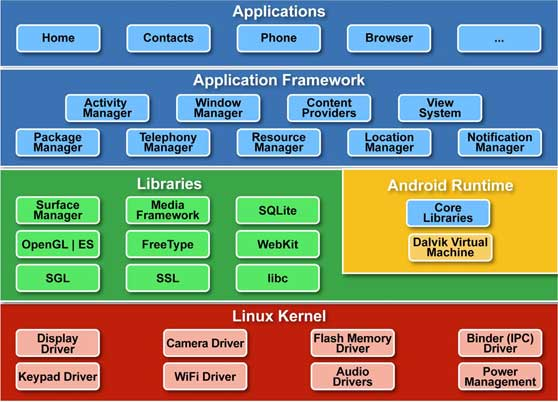
\includegraphics[scale=0.7]{img/android_architecture.jpg}
	\caption{Stos Androida, źródło: \cite{androidstack}}
	\label{fig:android_architecture}	
\end{figure}

Jeśli chodzi o~kod natywny(C/C++), to można na niego programować mniej więcej tak, jak na ``standardowego'' Linuxa. Ma podobny zestaw bibliotek. Część została włączona do systemu bez zmian. Ważnym wyjątkiem jest Bionic -- alternatywna implementacja biblioteki standardowej C (\emph{libc}). Google zdecydował się na jej przepisanie aby zoptymalizować ją pod urządzenia z~ograniczonymi zasobami oraz żeby uniknąć problemów licencyjnych związanych z~``infekcją'' przez licencję GPL (którą objęta jest \emph{libc}).

Trzeba powiedzieć, że pisanie programów w~C nie jest zalecanym sposobem pisania aplikacji na Androida. Podstawowym językiem jest Java. API dla tego języka dostarczane przez Google pozwala na budowanie programów, które klasyfikowane są jako aplikacje Androidowe. Te aplikacje przyjmuję postać paczek APK (Application Package). Mogą one być łatwo instalowane i~wykorzystywane przez zwykłych użytkowników.

Java, w~przeciwieństwie do np.~C nie jest kompilowana do kodu maszynowego, który może być wykonany przez procesor. Zamiast tego jest kompilowana do kodu bajtowego Javy (\emph{Java bytecode}), który abstrahuje od właściwości (takich jak architektura procesora) komputera, na którym ma być wykonany \cite{jvm}. Za wykonanie faktyczne wykonanie kodu na procesorze (zwane JIT -- z~ang. \emph{just-in-time compilation}) jest odpowiedzialna maszyna wirtualna Javy (ang.: \emph{Java Virtual Machine (JVM)}). JVM posiada różne wersje (wszystkie zgodne z~jedną specyfikacją) dopasowane do środowisk, w~których mają działać. Inna będzie potrzebna na Linuxa, inna na Windowsa. Ale każda z~nich powinna być w~stanie wykonać z~takim samym efektem taki sam kod Javy. Zatem teoretycznie można napisać jeden program, który bez żadnych modyfikacji będzie działał na całkowicie odmiennych systemach operacyjnych.

Na potrzeby Androida stworzona została nowa, otwarta JVM o~nazwie Dalvik. Dalvik jest zoptymalizowany na urządzenia mobilne. Faktycznie operuje na innym niż standardowy kod bajtowy, ale kod dla Dalvika uzyskuje się przez dodatkową kompilację (optymalizację) zwykłego kodu bajtowego (zilustrowane na rysunku \ref{fig:dalvik-compilation}). Teoretycznie, każdy język kompilowany do kodu bajtowego Javy (a~jest ich kilka, np. Scala) powinien móc być wykonany na Dalviku.
Poza tym, nowa maszyna wirtualna była potrzebna aby uniezależnić się od właściciela Javy (kiedyś Sun, obecnie Oracle). Narzędzia do język (jak kompilatory) i~standardowe odmiany JVM są darmowe, ale należą do Oracle, a~ich kod nie jest otwarty. Istnieją też, co prawda, alternatywne otwarte implementacje JVM, jak ta dostarczana z OpenJDK.

\begin{figure}
	\centering
		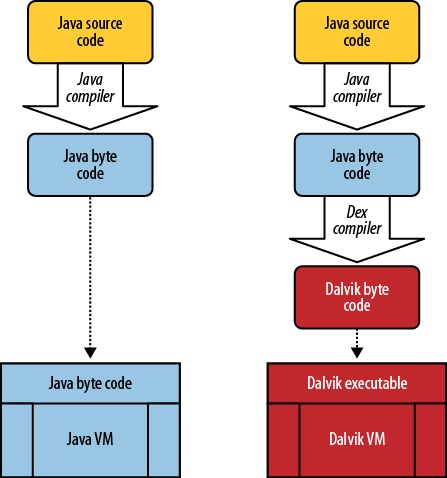
\includegraphics[scale=0.75]{img/dalvik-compilation.jpg}
	\caption{Porównanie standardowej kompilacji Javy z~kompilacją dla Dalvika. Źródło: \cite{learningandroid}}
	\label{fig:dalvik-compilation}
\end{figure}

Aktualnie istnieje już następca Dalvika -- Android Runtime (ART). Wprowadzono go jako alternatywną maszynę wirtualną w~ostatnim Androidzie (4.4)\cite{androidart}. W~kolejnej wersji systemu -- Androidzie L -- będzie już domyślny\cite{androidlpreview}. Jego głównym celem jest przyspieszenie wykonywania aplikacji. Osiąga to przez usprawnione odśmiecanie pamięcie (ang. \emph{garbage collection}) oraz przez wprowadzenie techniki określanej jako \emph{ahead-of-time compilation} (AOT), czyli kompilacja przed czasem (kontrast dla JIT). AOT polega na tym, że w~trakcie instalacji aplikacja (skompilowana do kodu Dalvika) jest kompilowana jeszcze raz, już na kod maszynowy dopasowany do urządzenia, na którym odbywa się instalacja. Przez to zużywane jest dodatkowe miejsce, ale aplikacja może się wykonywać szybciej, ponieważ jej kod nie musi być interpretowany przez JVM.

Java która jest dostępna na Androidzie niestety nie ma pełnego zbioru standardowych bibliotek (z~Javy SE). Między innymi, brakuje wielu części pakietu \emph{javax}. Niektóre rzeczy, za które były one odpowiedzialne to świadczenie i~konsumowanie usług internetowych (bycie serwerem lub klientem dla web service'ów), czy interfejsy użytkownika (Swing, AWT). W~zamian zostały dodane pakiety ułatwiające pisanie aplikacji pod Androida. Umożliwiają one komunikację aplikacji między sobą i~z~systemem, składowanie danych, dostęp do sensorów i~funkcji telefonu oraz wiele inne przydatnych działań\cite{androidpackage}. Wśród nich są też biblioteki odpowiedzialne za GUI Androida. Dzięki nim wszystkim ekosystem (programów) jest dość jednorodny i~ustandaryzowany.

Od jakiegoś czasu Java nie jest jedynym językiem, w którym można pisać aplikacje. Co prawda już kiedyś można dodać do APK bibliotekę C/C++ (pisaną przy użyciu NDK -- Native Development Kit\cite{androidndk}) i~wołać ją z~Javy, ale zawsze potrzebny był Javowy szkielet. Teraz można oznaczyć, że APK korzysta z~\emph{NativeActivity}\cite{androidnativeactivity}, co pozwala całość zaimplementować natywnie. 

Warto też powiedzieć, że każda aplikacja instalowana z~APK jest identyfikowana jako odrębny Unixowy użytkownik\cite{androidpermissions}. Dzięki temu można precyzyjnie zarządzać tym, do czego dana aplikacja ma dostęp, co zwiększa ogólne bezpieczeństwo systemu. W~systemach instalowanych na telefonach standardowo jest blokowane konto administratora systemu (\emph{root}). Użytkownik może je odblokować przez zabieg zwany rootowaniem.

Android nie ogranicza się do uruchamiania jedynie kodu napisanego w~C, C++ lub Javie (uznajmy je za języki ``standardowe''). Istnieje aplikacja działająca jako interpreter innych języków -- SL4A\cite{androidsl4a} -- która pozwala wykonywać skrypty napisane w~kilku językach, m.in.\ Python, Perl, Lua, JavaScript.\footnote{Inną aplikacją tego typu jest QPython (\url{http://qpython.com/}), która zawiera SL4A.}
Są też kompilatory tworzące kod bajtowy Dalvika z~języków inne niż standardowe (dla Androida). Tu przykładem jest Xamarin \footnote{\url{http://xamarin.com/}}, rozwiązanie umożliwiające pisanie w~C\# aplikacji na kilka platform, w~tym Androida.
Jednak zarówno SL4A i~Xamarin nie dają dostępu do wszystkich standardowych bibliotek. Jest tak dlatego, że użycie API Androida w~kodzie niestandardowego języka wymaga zmapowania do niego tychże API, co jest czasochłonne i~trudne do wykonania w~całości przez kogoś innego niż Google. Ponadto, niestandardowy dla Androida język, taki jak C\#, może mieć struktury, które nie dadzą się przetłumaczyć na kod bajtowy Javy. Tym samym nie będzie można go wykorzystać w~pełni. Odmiennym przypadkiem jest język Scala. Dzięki zgodności na poziomie kodu bajtowego (bo tak samo jak Java jest do niego kompilowana) Scala może być użyta do stworzenia kompletnego APK mającego dostęp do wszystkich bibliotek.

%Może wypunktowana lista ze wspieranymi językami? Tu macie języki i jak mocno i przez co są wspierane (może tabelka? nazwa | czy można całą aplikację w tym zrobić | jakiś opis, przez co dostarczane, uwagi). Dalej co ważniejsze opisane. Oczywiście jest więcej.

%\url{http://stackoverflow.com/questions/3316801/which-programming-languages-can-be-used-to-develop-in-android}
%\url{http://en.wikipedia.org/wiki/Android_software_development}
%https://github.com/jberkel/android-plugin
%https://github.com/jberkel/android-plugin/wiki/getting-started
%http://www.scala-sbt.org/release/tutorial/index.html

\subsection{.NET (TODO)}
Tu o .NETcie i o C\# (bo tego będę używał).
Jak .NET współpracuje z innymi środowiskami

\subsection{Porównanie cech Javy i C\#}
Porównać zdolności obu języków, znaleźć cechy nieprzetłumaczalne. Jak dużą zgodność można uzyskać teoretycznie?

\subsection{Python}
Pierwsza platforma jaką rozważałbym jako alternatywę dla podstawowych (Androida i .NETa) do implementacji mojej biblioteki. A to dlatego, że jest moją ulubioną. I może chodzić praktycznie na wszystkim.

Z drugiej strony, ten projekt może nie mieć dla niego sensu, bo jest duck typing. Nie musi być faktycznych związków między typami. Jeśli jakieś pola albo metody znajdą się w trakcie odpalania, to dany obiekt może być uważany za taki typ. Ale nie ma żadnego problemu z zachowywaniem zależności. Właściwie można wszystko wysłać bez etykiet jako proste JSONy. Nawet jak nie zachowamy nazw typów, to mniej więcej wszystko będzie działać.

Nie platforma a język, ale w sumie chodzi na wszystkim. I na windowsie, linuxie i androidzie. Lubię też w nim pisać. Można go sportować.

Wzmianka, że podstawowa implementacja pythona, której będę używał (albo i nie) nie korzysta z wielu procesorów.

\section{Zdalne wywoływanie kodu(TODO)}
Tu rozstaną opisane techniki umożliwiające zdalne wywoływanie kodu.

Zrób tak, żeby najpierw zarysować RPC, web servicy itp a dopiero potem wiązanie danych (żeby było wiadomo po co jest)

Dane (argumenty metod i~wartości przez nie zwracane) wymieniane pomiędzy klientem a serwerem będą miały postać obiektów (programowanie obiektowe). To znaczy, że typy dziedziczące i implementujące ten sam interfejs będą polimorficzne (źródło!). Często normalnie nie jest tak łatwo to osiągnąć w heterogenicznych środowiskach - ciężko o zachowanie związków między klasami po mapowaniu na drugi język

\subsection{Tłumaczenie danych}
Jaka jest problematyka przetłumaczenia danych/obiektów z jednego języka, platformy na drugą?
Nawet na niskim poziomie mamy little/big endian. Potem dochodzi jeszcze niezgodność kodów bajtowych platform wirtualnych.
Nawet jak się zapisze w XML, JSONie czy czymś innym to możemy stosować inne formaty, czy coś. Bindingi.

problemy komunikacji w heterogenicznych środowiskach (inne formaty danych, inne dostępne klasy i zasady działania obiektów, np. Type erasure)

Zgodność zapisu bajtowego obiektów w .NETcie, Javie i Dalviku (może inna niż w normalnej Javie, może pomiędzy maszynami wirtualnymi też różna). Gdyby wszystko było zgodne to nie trzeba by się było tak męczyć z szukaniem standardu opisu danych. Też type erasure wchodzi w grę (zapis bajtowy dwóch list różnych typów sprawdzić)

Niestety przekazywane obiekty nie mogą mieć żadnej większej logiki związanej z dostępem do swoich danych. O ile można zmapować pola klasy w jednym języku na pola w drugim, to przetłumaczenie metod dostępowych, które mają jakąś logikę (np. zmień licznik odczytań, kiedy czytam zmienną) w automatyczny sposób byłoby niemal niemożliwe (wymagałoby automatu rozumiejącego sens kodu -- programu programisty).

\url{http://json-schema.org/}\\
\url{http://bsonspec.org/}\\
\url{http://json.codeplex.com/}\\

\emph{JAKAŚ KSIĄŻKA O TYM?}

Ciężko o pełną swobodę w korzystaniu z obiektowości używanych przeze mnie języków, czyli Javy i C\#. Oba niby są obiektowe, ale przy przechodzeniu przez warstwę zdalną potrafią tracić tę właściwość.

\subsubsection{Serializacja}

\subsection{Transport danych}
Też bardzo szeroka dziedzina. Jak już się przetłumaczy, to zawsze trzeba jakoś przetransportować. Jak możemy przekazywać w ramach jednego kompa, jak pomiędzy kompami lokalnie, jak globalnie.
Celuję w globalnie, ale zwsze szerszą metodę można zastosować wężej (chociaż może nie być tak wydajna jak te węższe)

\emph{TEŻ PRZYDAŁBY SIĘ JAKIŚ ARTYKUŁ CHOCIAŻ}

\emph{TCP, PIPEy, SSL, HTTP, HTTPS, Webservicey, SOAP, REST, JSON}

\url{http://stackoverflow.com/questions/12450404/json-pojo-consumer-of-polymorphic-objects}

\subsection{RPC}
Ogólnie trochę o RPC. Że wiele technologii to RPC (Web service'y, CORBA), że to zawiera i tłumaczenie i transport.
Wywoływaniu kodu w innym procesie lub na innym kompie.

Czym jest programowanie obiektowe napisać, co to polimorfizm i dlaczego ważny. Web-servicey, XML-RPC, REST z JSONem i XMLem.

\url{http://www.infoq.com/articles/rest-soap-when-to-use-each}\\

\url{http://xmlrpc.scripting.com/default.html XML RPC}\\
\url{http://xmlrpc.scripting.com/spec.html}\\
\url{http://effbot.org/zone/xmlrpc-errata.htm}\\
Przejrzeć specyfikację, zobaczyć, z czym musieli sobie poradzić i wyczaić jak to wszystko mozna odwzorować w JSONie. Obczaić, jak sobie DataContractSerializer (też DataContractJsonSerializer) radzą. 

Service oriented architecture a remote procedure call? Jakie różnice? Czym będzie moje? A same web services?

\subsection{Binding}
A może najlepszym rozwiązaniem będzie generator customizowalnych bindingów (może nawet do JSONa) z wygodną konfiguracj)? Raz by się generowało mapowanie i wszystko działa na zawsze. 

NA TYM BĘDZIE DZIAŁAŁO TŁUMACZENIE KLAS
W WSDL poza opisami operacji realizowanych przez usługę znajdują się też pliki XSD opisujące wszystkie struktury danych (klasy), które będą wymieniane. Dla tego posiadając WSDL usługi możemy wygenerować wszystkie klasy potrzebne do stworzenia klienta usługi.

Złożony problem pojawia się wtedy, kiedy servicy mają działać w obie strony wykorzystując te same klasy danych. W bardziej skomplikowanych systemach rozproszonych może się pojawiać taka sytuacja. Załóżmy istnienie dwóch aplikacji: A i B. Są one napisane w różnych językach. Każda z nich udostępnia usługę zwracającą obiekt danych X. A korzysta z usługi wystawianej przez B, a B korzysta z usługi wystawianej przez A. Mimo tego, że obiekt X w obu aplikacjach będzie zawierał te same dane, to jednak jego kod będzie inny. Dlatego nie można mówić o jednej klasie X, a o dwóch. Nazwijmy je XA i XB. TUTAJ DALEJ WYTŁUMACZENIE PRZYKŁADU AŻ W KOŃCU DOJDZIEMY DO TEGO, ŻE TRZEBA NAPISAĆ KLASĘ W JEDNYM JĘZYKU, POTEM ZROBIĆ JEJ BINDING DO XSD I Z XSD DO DRUGIEGO JĘZYKA.

Problem przesyłania typów polimorficznych (coś przeczytać, może). 

\subsection{Web service'y i SOAP}
W sumie to przykład tłumaczenia danych  i transpotru.

SOAP ma faulty -- ważną rzecz w obiektowych językach (exception).

Jeden ze sposobów na zdalne wywoływanie kodu to usługi internetowe. Korzystając z otwartych standardów takich jak XML, SOAP, WSDL i UDDI umożliwiają integrację aplikacji poprzez Internet. XML jest używany do etykietowania danych, SOAP do ich pakowania i transferu (alternatywnie można używać też RESTa lub JSONa), WSDL opisuje interfejs usługi, a UDDI dostarcza spisu dostępnych usług (on nie leży w naszym obszarze zainteresowań). SOAP i WSDL są zapisywane przy pomocy XML. Web servicy używane są najczęściej do komunikacji aplikacji komercyjnych (np. serwery, portale) ze sobą lub z klientami. Pozwalają organizacjom na wymianę danych nie wymagając wiedzy o wewnętrznej strukturze informatycznej za firewallem.

W przeciwieństwie do tradycyjnych modeli przetwarzania typu klient – serwer, takich jak np. system stron internetowych, usługi internetowe nie mają graficznego interfejsu użytkownika. Służą one do dzielenia logiki biznesowej, danych i procesów poprzez sieć, przy pomocy jednolitego interfejsu programistycznego. To aplikacje się komunikują, nie użytkownicy. Programiści mogą, co prawda, dodać usługę internetową do aplikacji, która posiada GUI (np. aplikacja okienkowa lub strona internetowa) aby zaoferować zwykłym użytkownikom jej funkcjonalność.

Usługi internetowe pozwalają różnym aplikacjom wykonanych w różnych technologiach (np. całkowicie odmienne języki programowania) na porozumiewanie się ze sobą bez potrzeby czasochłonnego tworzenia kodu tłumaczącego. Nie ma też znaczenia to, czy obie aplikacje znajdują się na jednej maszynie, czy po drugiej stronie świata.
Usługi sieciowe na platformie .NET realizowane są w ramach WCF. Javie obecnym standardem jest JAX-WS.

co to webservicy i po co są?\\
do czego mogą się przydać na androidzie?\\
dlaczego ich nie ma? Chyba stwierdzili, że ogólne web servicey są za ciężkie i za bardzo obciążają (Windows phone też nie ma WCF)\\

Druga rzecz, którą chcę uzyskać to możliwość łatwego tworzenia programów współpracujących między wyżej wymienionymi platformami. Kiedy wywołujemy zdalny kod często trzeba przekazać mu jakieś parametry, często też chcemy otrzymać wartości zwrotne. Pomijając sam fakt transportu danych z jednej platformy na drugą stajemy przed problemem niezgodności typów danych. Wiemy, że na obu końcach będą użyte dwa różne języki, więc struktury danych nie będą kompatybilne. Trzeba temu zaradzić.
Ogólnie ujęte rozwiązanie dla powyższych problemów to serwer usług internetowych (ang. web services) wraz z narzędziami. Dzięki mechanizmowi usług sieciowych można wykonać dowolny kod na serwerze nie zależnie od technologii wykorzystywanych po obu stronach. Nie istnieje jeszcze (przynajmniej nie udało się znaleźć) serwer web service’ów dla Androida. Istnieją za to biblioteki pozwalające na przetłumaczenie klas z C\# na Javę.

WCF to webservice'y, a jednocześnie rekomendcja microsoftu na komunikację między procesami (co prawda na innym bindingu), tak że web servicey są dość uniwersalne i dobre nie tylko w dużej sieci do komunikacji między aplikacjami.

\subsection{JSON, YAML, AXON}
\url{http://intellimath.bitbucket.org/blog/posts/axon_overcomes_json.html}\\
Jakieś porównanie AXONa i JSONa. Jeśli AXON jest stabilny i wspierany na Androidzie i .NETcie (bardzo ważne) to powinienem go użyć, bo przecież parę problemów rozwiązuje.

Oznaczanie typów.

\subsection{REST}
Cośtam o RESTcie \url{http://www.oracle.com/technetwork/articles/javase/index-137171.html}\\
REST and POX \url{http://msdn.microsoft.com/en-us/library/vstudio/aa395208(v=vs.90).aspx}\\

Restful web services vs ``big'' web services: \url{http://www2008.org/papers/pdf/p805-pautassoA.pdf}\\

\chapter{Poszukiwanie rozwiązania}
Jak w ogóle dojść do tego  co i jak zrobić, żeby dało nam to, co mamy w celach? Jak się odnaleźć w tym wszystkim?
Wyjaśnić jak wytaczałem sobie drogę działania i jak metodyki dobierałem

Jak teoretycznie możnaby zrobić web service'y na Androidzie? Android jest tutaj przykładem ograniczonego systemu.
W sumie jakiś powód musięli mieć, żeby ich nie zamieszać. Jakie jeszcze dodatkowe usprawnienia byłyby do zrobienia (tłumaczenie klas)?

Najpierw zobaczmy, co jest.

Napisać, co jest potrzebne dla remotingu: jakaś tożsamość, adres obiektu, oznaczenia metod, argumentów.

Wprowadzenie nowego standardu nie jest dobrą rzeczą, chyba, że ma się ogromną rzeszę zwolenników lub poważne przesłanki. Kto wie, może takie mam. Ale na ogół lepiej kombinować istniejące rozwiązania tak, żeby zewnętrzne komponenty miały szansę na współpracę z nimi.

A czemu nie MONO/Xamarin?
\section{Pokrewne rozwiązania}
\label{existing_frameworks}
Tu o bibliotekach, frameworkach robiących to co chcemy albo rzeczy podobne.

Opisać jedną wspólną procedurę oceny dla każdej biblioteki: znalezienie w necie, instalacja, stworzenie prostej aplikacji, stworzenie bardziej skomplikowanej aplikacji (jakaś wymieniająca kilka ustalonych skomplikowanych drzew obiektów) łączenie z .NETem?

Konkretne porównania osiągów w rozdziale o eksperymentach (chociaż tutaj już zrobić porównanie wysiłku programisty, po prostu zamieścić je na końcu). Tutaj napisać o funkcjonalności żeby w ogóle wiedzieć, czy to czegoś warte i na ile mam się inspirować. Poza tym, może się okazać że jest już coś, co robi to, ca ja bym chciał zrobić.

Te wszystkie do serializacji i soapów rzeczy to są, tutaj nic nie ma. Wszystko co by się chciało to jest, ale na dużą Javę, albo na pythona (ciężko przeportować, nie wiadomo, czy da się na pewno) Apache Thrift, Google Protocol Buffers, ZeroMQ (http://stackoverflow.com/questions/8062212/difference-between-apache-thrift-and-zeromq)

Przy każdej technologii pokazać implementacje w WCF i Javie normalnej (bo ona będzie takim punktem odniesienia) i zrobić porównania prędkości, bezpieczeństwa itp.

Każdy framework opisać ile plików, jaką objętość trzeba ściągnąć. Ile kroków instalacji, ile rzeczy trzeba zrobić, żeby wystawić jakiś helloWorld serwis i jakiś serwis z własnymi danymi. Zrobić zestawienie frameworków (tabelę), czy pozwalają na wystawianie serwisów, czy tylko korzystanie. Czy pozwalają na polimorficzne argumenty.

GSOAP

Python EVE (Rest framework)

\url{http://www.webopedia.com/TERM/W/Web_Services.html}\\
\url{http://thrift.apache.org/static/files/thrift-20070401.pdf}\\
reliable sessions (w sumie też by mi się przydał jakiś mechanizm, który umożliwi komunikację w niestabilnym środowisku Internetu)\\
\url{http://blogs.msdn.com/b/shycohen/archive/2006/02/20/535717.aspx}\\
\url{http://docs.xamarin.com/guides/cross-platform/application_fundamentals/web_services}\\
\url{http://wsme.readthedocs.org/en/latest/}\\

Apache Thrift, Google Protocol Buffers, ZeroMQ (\url{http://stackoverflow.com/questions/8062212/difference-between-apache-thrift-and-zeromq})\\
\url{http://thrift.apache.org/static/files/thrift-20070401.pdf}\\
\url{http://blogs.msdn.com/b/shycohen/archive/2006/02/20/535717.aspx}\\
Xamarin\\
\url{http://docs.xamarin.com/guides/cross-platform/application_fundamentals/web_services/}\\

JiBX!!! Tworzenie klas ze schemy i robienie wsdl z javy\\
Wsdl2Java: tworzenie klas z wsdl, głównie chodzi o klasy danych\\

Serializacja:\\
\url{http://simple.sourceforge.net/}\\
\url{http://code.google.com/p/dbdroid-remoting/} - klient web serviców serializujący i deserializujący xmle\\
Generacja javovego kodu z bindingu:\\
XSD2Java – generuje kod java z xsd. Mocno niedorobione.\\
Inne:\\
\url{http://stackoverflow.com/questions/6920175/how-to-generate-java-classes-from-wsdl-file}\\
\url{http://blog.tourgeek.com/2011/12/xml-data-binding-for-java-on-android.html}\\
PODOBNE, ALE NIE PRZYDATNE:\\

\url{http://forum.springsource.org/showthread.php?129058-Spring-Remoting-for-Android}\\
\url{http://www.themidnightcoders.com/fileadmin/docs/java/v4/index.html?android}\\
\url{http://developer.android.com/guide/components/aidl.html} - AIDL, androidowa komunikacja między procesami\\


\subsection{WCF}
\url{http://msdn.microsoft.com/en-us/library/system.runtime.serialization.json.datacontractjsonserializer.aspx}\\
Generowanie z JAX-WS nie do końca działało.

\subsection{JAX-WS}
Niestandardowe podejście z użyciem JSONa zamiast XMLa\url{http://jax-ws-commons.java.net/json/}\\

\subsection{Jackson}
\url{http://www.cowtowncoder.com/blog/archives/2010/03/entry_372.html}\\
\url{http://stackoverflow.com/questions/8368873/deserialize-json-string-generated-from-net-using-jackson}
\url{http://stackoverflow.com/questions/10329706/json-deserialization-into-another-class-hierarchy-using-jackson}
\url{http://stackoverflow.com/questions/14454028/polymorphic-serialization-of-collections-with-custom-serializer-in-jackson}
\url{http://stackoverflow.com/questions/12350571/how-can-i-change-global-type-information-format-in-jackson}

sprawdzić jak się wymienia ze wszystkim opisanym adnotacjami (dodać jeszcze rozszerzenie defaulttyperesolvera), wtedy sprawdzić mixed iny; lista objectów, na którą wpakuję stringi i inty

\subsection{Restlet}
\url{http://restlet.org/learn/tutorial/2.1/#/docs_2.0/13-restlet/275-restlet/266-restlet.html}\\
\url{http://wiki.fasterxml.com/JacksonHowToIgnoreUnknown}\\

\subsection{Spring}
\subsection{Crest}
\subsection{Ksoap}

\subsection{I-jetty}
Jest to serwer, może ma jakiś kontener Web-serviceów?

\subsection{Porównanie możliwości tych technologii}

Jakieś niestandardowe (third-party) narzędzia tworzące WSDLa z Javy i .NETa i z WSDLa klasy? To samo do schemy i ze schemy?

\section{Moje pomysły na rozwiązanie}
Wymienić, zrobić POCe, porównać, wybrać i uzasadnić wybór. Wypracować jaką metodę odcięcia pracy na POCem? Że jak będę widział, że da się coś zrobić, ale jest to za trudne to kończyć pracę.

Namespace'y są ważną rzeczą w SOAPie. Ja twierdzę, że nie są potrzebne w tak rozbudowanej formie. Może być jedno standardowe nazewnictwo z kropkami. Zakładam taki jakby jeden globalny namespace na oba runtime'y (klient i serwer). Fakt, że nawet jedna strona może mieć kilka przestrzeni nazw (parę class loaderów albo assembly cache'y) ale nie chcę tego robić z uwagi n utrudnienia w integracji (tu można napisać jakby to mogło wyglądać, ale nie trzeba, mogę po prostu to olać).

Napisanie wszystkiego w C, Javie albo nawet Pythonie. Z czym by się to wiązało. Chcemy żeby było łatwo, co by trzeba było zrobić wtedy?
Podłączanie się pod istniejące rozwiązania Axis w C, portowanie Pythona, tłumaczenie JibXem

Zdecydowałem się to zrobić web servicami opartymi o SOAP, blabla, jednolite dla javy tej i normalnej
Tu już konkretnie jakie biblioteki, jak konkretniej to będzie wyglądać

Tyson? Typed JSON?

a)	Rozpoznanie istniejących rozwiązań dotyczących wiązania danych (ang. data binding) z XML oraz wystawiania usług sieciowych (ang. web services) w językach Java oraz C++.
Zaprojektowanie i wykonanie biblioteki pozwalającej na przyjmowanie, przetwarzanie, tworzenie i wysyłanie wiadomości SOAP, generowanie plików WSDL na bazie kodu oraz na wiązanie danych z języka C\# do języka Java z zakresem bibliotek dostępnym na Androidzie. Akceptowalne jest również stworzenie biblioteki, w której komunikacja oparta zostałaby o protokół TCP/IP i serializację obiektów do XML tak, by były rozumiane zarówno przez kod w języku Java, jak i w języku C\#.

Użyć w Pythonie Flaska do tłumaczenia JSONa? Albo jakiegoś innego tłumacza python-JSON.

Jak jest? \\
JAVA dla przykładu \\
Co trzeba robić w javie			Co trzeba robić w C\# \\
ANDROID \\
Co trzeba zrobić na androidzie		Co trzeba robić w C\# \\

Jak może być? \\
Co robimy, żeby tak było? \\
Co trzeba wtedy robić na androidzie	Co w C\# \\

Może zamiast tylu podsekcji najpierw wyliczenie, krótki opis i decyzja, czy należy się tym zajmować? Dopiero te, które wydawałyby się bardziej interesujące dostają swoją własną podsekcję.

\subsection{własna metoda oparta o JSON z oznaczaniem typów}
Póki co wiem, że będzie JSON z opisanymi typami. Kanał komunikacyjny powinien być dowolny. 

Może zamiast równoważnych implementacji na pythona, C\# i javę zrobić tylko pythona i wrappery w jythonie i iron pythonie?

\subsection{serwer web serviców z narzędziami do generacji kodu itp}
Generator wsdl na Androida + tworzenie bindingów do xsd + Parsowanie SOAPów

JiBX!!! Tworzenie klas ze schemy i robienie wsdl z javy
Wsdl2Java: tworzenie klas z wsdl, głównie chodzi o klasy danych

Weryfikacja: tworzę graf w xmlu. Są obiekty, które mogą mieć dzieci (tablice, listy). Próbuję wygenerować C\# dla porównania. Zapisuję grafy, które nie działają (w trakcie automatycznych testów). Zrobić wizualizator grafów.

Co by trzeba było po kolei zrobić w normalnej javie? (tłumaczenia do xsd, ujednolicanie namespaców, mamy do czynienia z jakimiś ArrayOfString, dziedziczenie chyba słabo działa przy generacji, nie da się używać DataContractSerializera żeby nie serializować części klas ogólnie syf, ale wszystko udokumentować). 

\subsection{Własny serwer REST}
Tu dyskusja o implementacji serwera RESTowego na Androidzie \url{https://groups.google.com/forum/?fromgroups=#!topic/android-developers/vgkXg1P8iBg}

\subsection{remoting przez serializację}
Po prostu serializujemy tak samo/

\subsection{portowanie rozwiązań w C na Androida?}
Axis. Może częściowe używanie go spod javy. W sumie można sportować też jakieś inne rzeczy. Np.\ pythonowe web service'y (pyro, twisted).

Sprawdzić Python Remote Objects (Pyro) na pythonie 2, 3 (też na warstwie skryptowej Androida). Porównać z Twistedem, napisać o próbach portowania wymaganych bibliotek w C na Androida. \url{http://pythonhosted.org/Pyro4/intro.html#performance}

sl4a, py4a, kompilacja na ubuntu z użyciem NDK i Cythona
distutils.core zamienić na setuptools w setup.py

\subsection{Zcentralizowane pseudo web servicy (albo nawet i nie)}
Też potrzebny serializator / deserializator + bindingi. To był ten pomysł, że to komp pinga serwer (Androida), żeby ten sobie pobrał rozkaz i to Android woła web service na kompie. Trzeba by było używać Ksoap albo innego ścierwa. Zobaczyć, czy to w ogóle miałoby sens. Czy tymi Ksoapami da się coś sensownie zrobić.

\subsection{Wybrane rozwiązanie}
Jakie i dlaczego?

Dlaczego nie Soap, bindingi itp.?


\chapter{Projekt systemu i elementy implementacji}
W~tym rozdziale zaprojektuję oprogramowanie realizujące cele opisane w~punkcie~\ref{lib-requirements}.
Zaproponuję sposób realizacji, możliwości i~ograniczenia poszczególnych jego elementów. Dla części komponentów stworzę prototypy.

\section{Specyfikacja wymagań systemowych (SWS)}
Z~celów tej pracy zawartych w~punkcie~\ref{lib-requirements} stworzyłem standardową listę konkretnych wymagań dla zespołu inżynierów, czyli mnie samego.
Organizując niniejszą sekcję wzorowałem się na specyfikacji wymagań systemowych opisanej w~prezentacji ,,Inżynieria Wymagań'' Jarosława Kuchty, z~przedmiotu ,,Dokumentacja i~Jakość Oprogramowania''\cite{kuchta}.


\subsection{Wstęp i~opis informacyjny}
Jako rozbudowana sekcja wstępu SWS oraz ,,szczegółowy opis problemów do rozwiązania'' służyły poprzednie rozdziały niniejszej pracy.


\subsubsection{Diagram przepływu najwyższego poziomu}
Diagram~\ref{fig:project-overview} przedstawia ogólne działanie systemu w~trakcie wywoływania zdalnej metody. Jest to główna funkcja mojego projektu. Funkcja drugorzędna -- tłumaczenie danych, również została ujęta.


Widoczny na schemacie klient jest jednym z~wielu, które mogą być stworzone przez kod korzystający z~mojej biblioteki.
Obiekt każdego klienta spełnia jakiś zadany interfejs. Robi to przez opakowywanie parametrów, zaadresowanie ich, wysłanie do obiektu faktycznie wykonującego kod i~odebranie wyniku.
Interfejs klienta i obiektu zdalnego są zgodne, chodź napisane w~różnych językach na różne platformy. Aby zminimalizować nakład pracy programisty, najlepiej byłoby, gdyby interfejs po stronie klienta (.NET) był generowany z~wersji serwerowej (Java, Android).
Tak samo jak w~przypadku interfejsów wygląda sprawa klas przekazywanych do metod jako parametry -- także muszą być zgodne, najlepiej automatycznie tłumaczone.
Typy przetłumaczone na schemacie oznaczone są apostrofem.
Kod kliencki nie musi zawierać tłumaczenia implementacji zdalnych interfejsów.
Współdzielone definicje klas danych i~interfejsów są niezbędne, aby uzyskać polimorfizm metod zdalnych.

Serwer jest tworzony przez kod kliencki i~nasłuchuje na żądania na zadanym interfejsie sieciowym. Może to być dowolna technologia pozwalająca na dwustronne wysyłanie wiadomości, np.\ TCP, HTTP, SSL/TLS, czy też strumienie w~pamięci (rozwiązanie lokalne).
Na schemacie serwer posiada tylko jeden obiekt zdalny klasy \texttt{Implementacja A}, ale faktycznie może posiadać ich wiele.

\begin{figure}
	\centering
		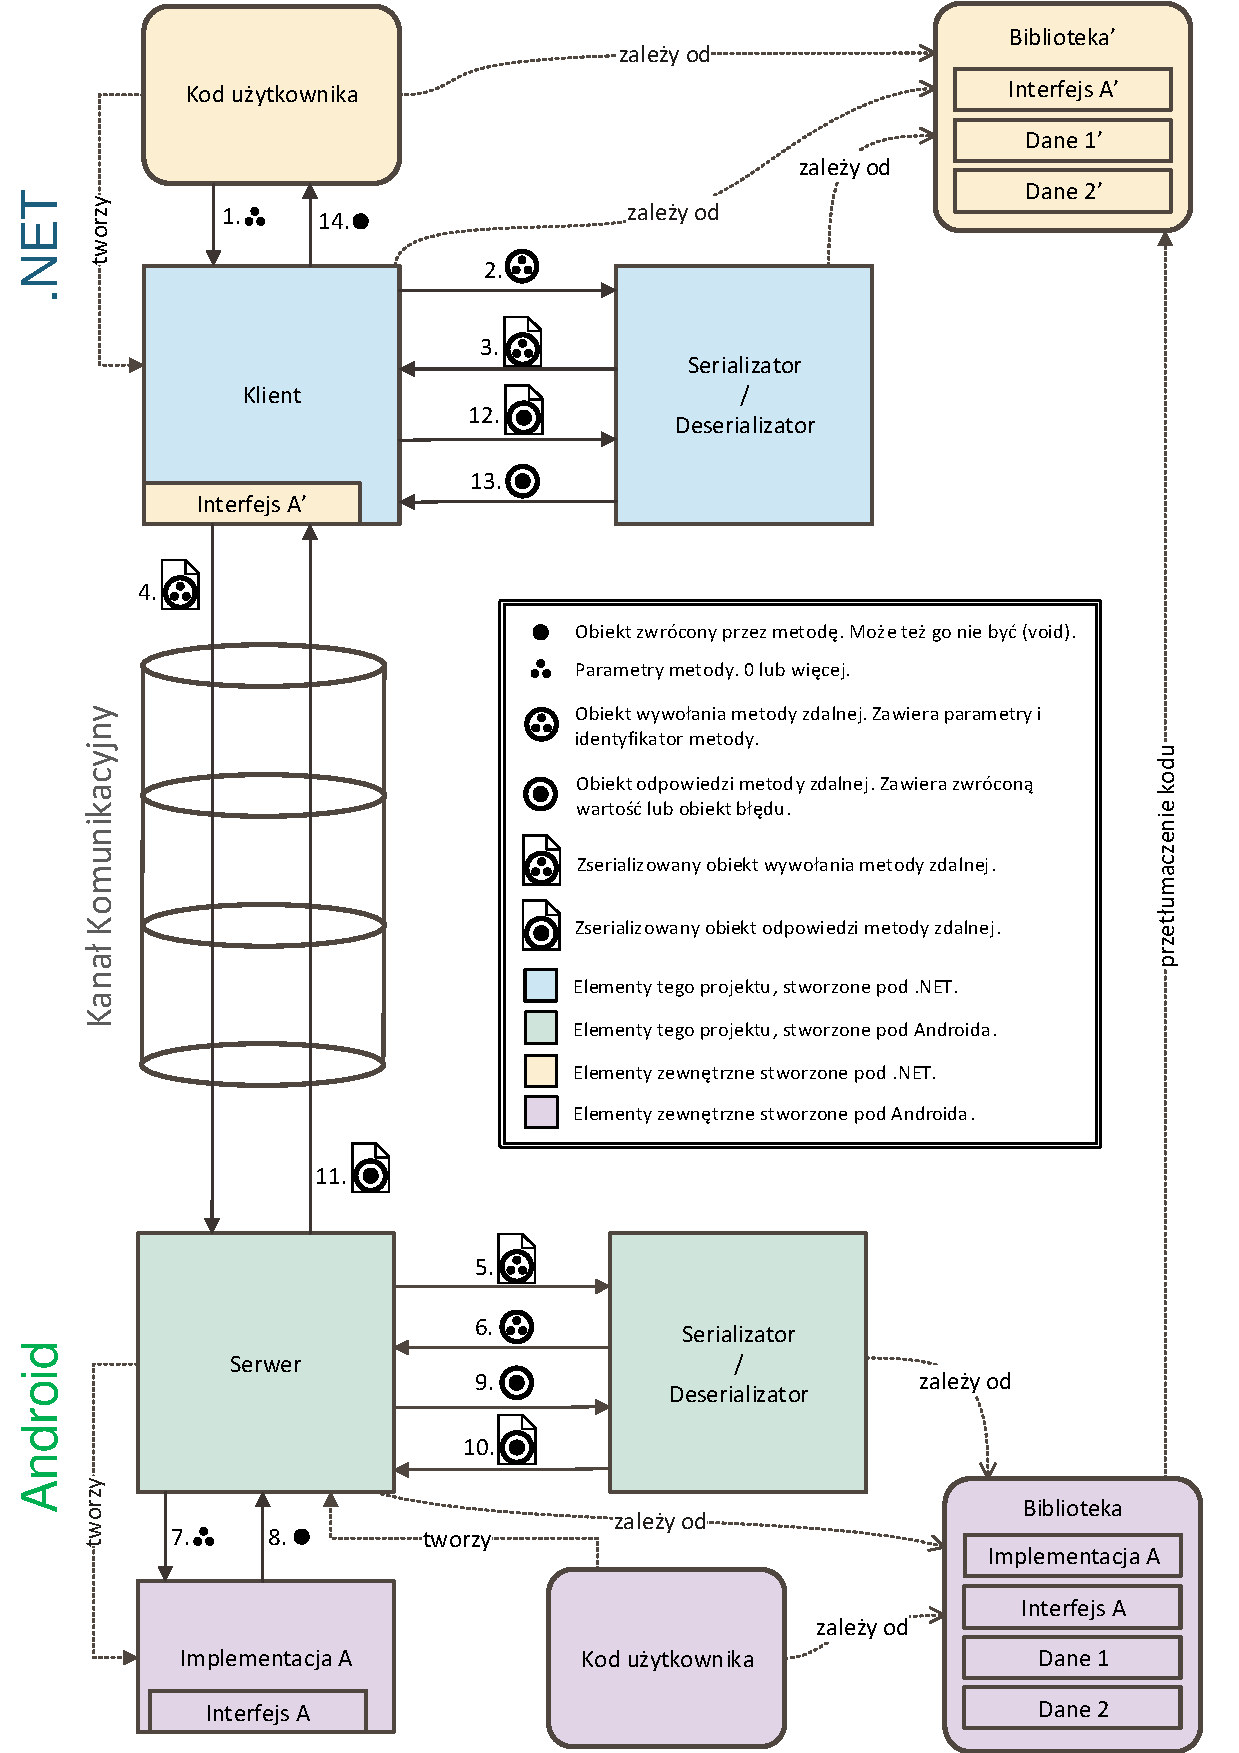
\includegraphics[scale=0.8]{img/schematy/schemat-dzialania-magisterki.pdf}
	\caption{Ogólny schemat projektu.}
	\label{fig:project-overview}
\end{figure}


\subsubsection{Reprezentacja zawartości informacyjnej}
Nie można właściwie mówić o~zawartości informacyjnej systemu, ponieważ takiej nie będzie.
Przez mój system dane będą jedynie przepływać.


\subsubsection{Opis interfejsów systemowych}
\begin{itemize}
	\item Jako, że to, co tworzę będzie kolekcją bibliotek Javy i~C\# będą one mogły być ładowane, a~ich klasy wykorzystywane przez zewnętrzne aplikacje.
	\item Niezależne narzędzie do generacji kodu będzie opatrzone w~interfejs linii poleceń.
\end{itemize}


\subsection{Wymagania funkcjonalne}
% WYMAGANIA POMIJANE:
% reliable sessions (w sumie też by mi się przydał jakiś mechanizm, który umożliwi komunikację w niestabilnym środowisku Internetu)
% \url{http://blogs.msdn.com/b/shycohen/archive/2006/02/20/535717.aspx} \\

\subsubsection{Ogólne}

\begin{description}
\itemtitle{Serializacja danych z zachowaniem informacji o typach}
Zserializowane reprezentacje obiektów muszą zawierać informacje o~typach wtedy, kiedy nie wynika ona jednoznacznie z~kontekstu.
Np.\ przy zwracaniu ze zdalnej metody obiektu klasy dziedziczącej po tym, zdeklarowanym w~interfejsie tejże metody.
To wymaganie dotyczy zarówno strony klienta jak i~serwera.
Deserializacja powinna być komplementarna i~ze stworzonych reprezentacji odtwarzać obiekty o~odpowiednich typach i~z~poprawnymi danymi.
Taka metoda serializacji i~deserializacji jest warunkiem działania polimorficznych metod.

\itemtitle{Tłumaczenie kodu}
Zrealizowane jako niezależne narzędzie.
Tłumaczenie kodu zmniejszyłoby nakład pracy programisty, który bez tego musiałby sam stworzyć odpowiadające klasy danych w~obu językach.
Klasy i~pola nie znajdujące odpowiednika są pomijane w~trakcie tłumaczenia.
Tłumaczenie powinno się odbywać z~Javy do C\#, ponieważ w~Javie będzie więcej kodu (kod implementacji zdalnych metod).
%Jeśli w danej klasie są inne klasy z zewnętrznej biblioteki, to trzeba też przetłumaczyć te. Trzeba dostarczyć kod wszystkich.
%Jeśli jedno ogniwo jest nieprzetłumaczalne to można pominąć pole z ostrzeżeniem.
\end{description}

\subsubsection{Serwer}

\begin{description}

\itemtitle{Komunikacja z~klientem}
Serwer powinien nasłuchiwać na żądania od klientów na zadanym dwustronnym kanale komunikacyjnym.
Konkretny typ kanału (TCP, SSL, HTTP, itp.) nie jest ważny.
Może przyjmować wywołania metod i~przekierowywać je do obiektów zdalnych (względem klienta).
Przekazuje do klientów zwracane wartości.

\itemtitle{Wystawianie metod publicznych zadanych obiektów ,,na zewnątrz''}
Kod serwera ma przyjmować dowolny obiekt i~umożliwiać zdalnym klientom wywoływanie jego publicznych metod.
Parametry tych metod muszą być przetłumaczalne na kod klienta.

% Można się też zastanowić nad singletonami.
\itemtitle{Tworzenie zdalnych obiektów na życzenie klienta}
Po otrzymaniu specjalnego żądania kod serwera powinien stworzyć obiekt implementujący zadany interfejs i~zwrócić jego identyfikator. Klient będzie mógł wywoływać zdalnie metody na stworzonym obiekcie.

\itemtitle{Niszczenie zdalnych obiektów na życzenie klienta}
Specjalne żądanie zawierające identyfikator obiektu powinno powodować jego zwolnienie i~uniemożliwienie z~nim dalszej komunikacji.

\itemtitle{Polimorfizm parametrów metod zdalnych}
Metody zdalne muszą obsługiwać parametry wszystkich typów zgodnych ze spodziewanym. Dla przykładu, metoda przyjmuje parametr typu A, więc powinna przyjąć też parametry wszystkich typów dziedziczących po A.

\itemtitle{Przeciążanie metod zdalnych}
Metody zdalne mogą być przeciążane, tj.\ dwie metody mogą mieć tę samą nazwę, ale inny zestaw parametrów.

\itemtitle{Komunikacja z systemem Android}
Obiekty zdalne muszą mieć możliwość wywoływania metod z~API Androida.

\end{description}

\subsubsection{Klient}

\begin{description}

\itemtitle{Tworzenie obiektów klienckich}
Biblioteka po stronie .NET musi być w~stanie dynamicznie stworzyć obiekt klienta dla obiektu zdalnego.
Każdy klient spełnia jakiś zadany interfejs.

\itemtitle{Nawiązywanie sesji z~serwerem}
Obiekt klienta nawiązuje kontakt z~serwerem poprzez dowolny dwustronny kanał komunikacyjny (na którym serwer nasłuchuje).
Następnie żąda od serwera stworzenia dla siebie zdalnego obiektu.
Wszystkie metody z~interfejsu zdalnego wywoływane na kliencie są przekazywane do jednego obiektu zdalnego.
Zwolnienie obiektu klienta powoduje zwolnienie obiektu zdalnego.

\itemtitle{Konsumowanie polimorficznych metod zdalnych}
Klient wykonuje metody implementowanego przez siebie interfejsu przez delegację (i~wysłanie) ich do obiektu zdalnego.
Wysłanie poprzedzane jest serializacją, podczas której muszą zostać zachowane informacje o~typach parametrów oraz ich ewentualnych obiektach składowych.

\end{description}


\subsection{Wymagania niefunkcjonalne}

\begin{description}

\itemtitle{Serwer na Androidzie}
Kod serwera musi działać na platformie Android.

\itemtitle{Klient w~.NET pod Windows}
Kod klienta musi działać na platformie .NET\@.

\itemtitle{Wydajność serwera}
Nie musi być duża, jako, że nie jest priorytetem projektu. Wystarczy jednoczesna obsługa pięciu (5) klientów.

\itemtitle{Rozszerzalność metod zdalnych bez ingerencji w oryginalny kod}
Funkcjonalność metod zdalnych powinna być rozszerzalna bez ingerencji w~ich kod dzięki mechanizmom programowania obiektowego.
Przykładem jest możliwość przyjmowania przez metodę zdalną obiektu klasy dziedziczącej po spodziewanym typie parametru, bez potrzeby jakiejkolwiek ingerencji w~kod metody, aby mogła rozumieć nową klasę.
Jednak definicja nowej klasy musi być dostępna zarówno dla klienta, jak i~serwera.

\itemtitle{Łatwość użytkowania}
Budowanie i~korzystanie z~bibliotek, które powstaną w~trakcie realizacji tego projektu, powinno być proste i~intuicyjne.

\end{description}



\section{Używana konfiguracja sprzętowa i~narzędzia}
\label{system-configuration}
Przed przystąpieniem do omawiania komponentów rozwiązania warto wspomnieć o~tym, na jakiej konfiguracji sprzętowej oraz przy pomocy jakich narzędzi były wytwarzane kod i~tekst niniejszej pracy. Na tej samej konfiguracji wykonywane były testy \emph{frameworków} w~rozdziale~\ref{similar-technologies}.

\begin{description}
\itemtitle{System operacyjny}
Windows 7 Professional x64. Cały kod i~tekst pracy powstał na tej maszynie. Na niej był też osadzony emulator Androida.

\itemtitle{Emulator Androida}
Ściągnięty razem z~IDE Eclipse zmodyfikowanym do pracy z~Androidem\footnote{Do ściągnięcia ze strony \url{http://developer.android.com/sdk/index.html}}.
Jest to standardowy emulator od Google\footnote{Alternatywnym emulatorem jest Genymotion (\url{http://www.genymotion.com/}), polecany na stronach Xamarina.}.
Emulowany był Android 4.4.2 (poziom API Androida w~tej wersji to 19). Reszta konfiguracji emulowanego urządzenia: typ obrazu~-- \emph{ARM EABI v7a}, urządzenie~-- Nexus S, RAM~-- 512MB, \emph{VM Heap}~-- 32MB, wewnętrzna pamięć~-- 200MB, karta SD~-- 50MB, zaznaczona opcja użycia GPU hosta.
%Używam ARMowego, bo więcej telefonów jest właśnie na nim. Zdażają się też drobne rozbieżności działania niektórych niskopoziomowych aplikacji względem obrazu na architekturę x86 (\emph{Intel x86 Atom}).

\itemtitle{Eclipse 4.2.1 z~wtyczką ADT}
Przy jego użyciu stworzona jest przykładowa aplikacja serwerowa, a~także inne aplikacje powstające w~trakcie testów \emph{frameworków} (rozdział~\ref{similar-technologies}). ADT -- \emph{Android Development Tools}, to wtyczka umożliwiająca tworzenie kodu na Androida.

\itemtitle{NetBeans 7.4}
Kod Javy niewymagający Androida do działania powstawał w~nim.

\itemtitle{Visual Studio 2013 Ultimate}
Pod nim powstawał cały kod C\#.

\itemtitle{Tortoise GIT}
GIT jest systemem kontroli wersji w~którym trzymany jest kod oraz tekst tej pracy. Wykorzystywany przeze mnie klient to TortoiseGit\footnote{\url{https://code.google.com/p/tortoisegit/}}. Repozytorium znajduje się pod adresem \url{https://github.com/butla/SimRemo}.

\itemtitle{\LaTeX}
Tekst pracy pisany jest przy pomocy technologii \LaTeX. Jako edytor wykorzystywany jest program TeXnicCenter\footnote{\url{http://www.texniccenter.org/}}.
\end{description}

%Do testów wymagane jest przekierowanie portu TCP hosta do portu TCP emulatora. Do tego należy użyć komendy:
%\begin{lstlisting}[language=bash]
%adb forward tcp:1666 tcp:1666
%\end{lstlisting}
%Adb to komenda z narzędzi instalowanych z Eclipsem.



\section{Częściowa implementacja}
Tutaj przedstawię zaimplementowaną część zaplanowanego projektu. Całość okazała się zbyt obszerna na jedną pracę dyplomową. W~dalszej części rozdziału dokładniej przedstawię poszczególne elementy systemu (zarówno te zaimplementowane jak i~nie) oraz wyzwania z~nimi związane. Uzasadnię też metody ich implementacji.

\subsection{Spełnienie wymagań systemowych}
Spełnienie zdefiniowanych wymagań systemowych przez stworzoną implementację zostało przedstawione w~tabeli~\ref{tab:requirements-fulfilment}.

\begin{table}[htbp]
	\centering
		\begin{tabular}{ | c | c | c | c | }
			\hline
				\textbf{Nazwa wymagania} & \textbf{Typ wymagania} & \textbf{Obszar} & \textbf{Wykonanie}\\
				\hline \hline
				Serializacja danych z zachowaniem informacji o typach & Funkcjonalne & Ogólne & +\textasciitilde\\
				\hline
				Tłumaczenie kodu & Funkcjonalne & Ogólne & +\\
				\hline
				
				Komunikacja z~klientem & Funkcjonalne & Serwer & +\\
				\hline
				Wystawianie metod publicznych zadanych obiektów ,,na zewnątrz'' & Funkcjonalne & Serwer & + \\
				\hline
				Tworzenie zdalnych obiektów na życzenie klienta & Funkcjonalne & Serwer & -- \\
				\hline
				Niszczenie zdalnych obiektów na życzenie klienta & Funkcjonalne & Serwer & -- \\
				\hline
				Polimorfizm parametrów metod zdalnych & Funkcjonalne & Serwer & + \\
				\hline
				Przeciążanie metod zdalnych & Funkcjonalne & Serwer & + \\
				\hline
				Komunikacja z systemem Android & Funkcjonalne & Serwer & + \\
				\hline
				
				Tworzenie obiektów klienckich & Funkcjonalne & Klient & +\textasciitilde \\
				\hline
				Nawiązywanie sesji z serwerem & Funkcjonalne & Klient & -- \\
				\hline
				Konsumowanie polimorficznych metod zdalnych & Funkcjonalne & Klient & + \\
				\hline
				
				Łatwość użytkowania & Niefunkcjonalne & Ogólne & +\textasciitilde \\
				\hline
				Serwer na Androidzie & Niefunkcjonalne & Serwer & + \\
				\hline
				Rozszerzalność metod zdalnych bez ingerencji w oryginalny kod & Niefunkcjonalne & Serwer & + \\
				\hline
				Wydajność serwera & Niefunkcjonalne & Serwer & + \\
				\hline
				Klient w .NET pod Windows & Niefunkcjonalne & Klient & + \\
				\hline
		\end{tabular}
	\caption[Spełnienie wymagań systemowych.]{Spełnienie wymagań systemowych. ,,+'' oznacza, że wymaganie jest spełnione; ,,+\textasciitilde'', że zostało spełnione ale wymaga komentarza; ,,--'' że nie zostało spełnione.}
	\label{tab:requirements-fulfilment}
\end{table}

Komentarz do niespełnionych wymagań:
\begin{description}
\itemtitle{Tworzenie zdalnych obiektów na życzenie klienta}
Mechanizm w~ogóle nie zaimplementowany. Zdalne obiekty (serwisy) działają jako singletony; każdy obiekt musi być stworzony przez serwer i~powiązany z~unikatowym adresem. Wszystkie żądania wysłane na jeden adres są obsługiwane przez jedną instancję serwisu.

\itemtitle{Niszczenie zdalnych obiektów na życzenie klienta}
Ponieważ nie zostało zaimplementowane tworzenie obiektów na życzenie nie ma sensu implementować usuwania.

\itemtitle{Nawiązywanie sesji z serwerem}
Sesje miały być nawiązywane na zasadzie przyznawania każdemu klientowi osobnej instancji serwisu. Ponieważ klient nie może stworzyć obiektu zdalnego na serwerze to sesje nie mogą być zaimplementowane.
\end{description}

Są jeszcze wymagania zaimplementowane, które jednak wymagają komentarza:
\begin{description}
\itemtitle{Serializacja danych z zachowaniem informacji o typach}
Nie ma wsparcia dla oznaczania typów kolekcji: tablic, list, słowników itp.
\itemtitle{Tworzenie obiektów klienckich}
Kiedy zdalna metoda rzuci wyjątek to pewien wyjątek jest rzucany przez metodę obiektu klienckiego. Nie jest to jednak przetłumaczony obiekt wyjątku rzuconego po stronie serwera, a~wyjątek typu \texttt{JsonRpcException} zawierający tekstowy zapis tego oryginalnego.s

\itemtitle{Łatwość użytkowania}
Ustawianie słownika typów mogłoby się odbywać za pośrednictwem pliku konfiguracyjnego. Aktualnie odbywa się w~kodzie, przy pomocy wywołania statycznej metody, która może być trudna do znalezienia, jeśli się nie wie gdzie szukać.
\end{description}


\subsection{Zasady działania}
Możliwości zaimplementowanego systemu to:
\begin{itemize}
	\item serwowanie publicznych metod wybranych obiektów zdalnie, z~Androida;
	\item dynamiczne tworzenie obiektów klienckich z~poziomu .NET; obiekty implementują zadany (zdalny) interfejs;
	\item polimorfizm parametrów metod zdalnych, ale tylko jeśli są pojedynczymi obiektami, a~nie kolekcjami;
	\item przeładowywanie metod zdalnych.
\end{itemize}

W~ogólności system pozwala na wystawienie publicznych metod zwykłego javowego obiektu ,,na zewnątrz'' systemu Androida.
Taki wystawiany obiekt zwany jest od teraz obiektem zdalnym.
Program na Androidzie wystawiający obiekty zdalne działa jako serwer, konkretnie serwer JSON-RPC -- standardu zdalnego wywoływania metod opartego o~JSON, opisanego w~punkcie~\ref{json-rpc}.

System zawiera też klienta JSON-RPC pod .NET. Przy jego pomocy można dynamicznie, wywołaniem jednej metody, stworzyć obiekt spełniający zadany interfejs będący klientem obiektu zdalnego.
Dla przykładu: kod na Androida zawiera interfejs \texttt{TestService} i~klasę \texttt{TestServiceImpl} go implementującą, obie stworzone przez hipotetycznego użytkownika mojego systemu, a~nie będące jego częścią.
Po stronie .NET musi znajdować się interfejs lustrzany dla \texttt{TestService} z~Javy (Androida), czyli posiadający tak samo nazwane metody z~analogicznymi parametrami.
Na bazie tego interfejsu tworzony jest obiekt kliencki dla obiektu zdalnego. Można na nim wykonywać metody interfejsu \texttt{TestService} tak jak na zwykłym lokalnym obiekcie -- zwracane wartości będą normalnymi obiektami.

Można wywoływać

Struktura tego, co zostało zaimplementowane przedstawiona jest na schemacie~\ref{fig:implementation-overview}.
Dokładniejsza struktura przygotowanej biblioteki .NET przedstawiona jest na diagramie~\ref{fig:dot-net-classes}.
Przygotowana przeze mnie część Androidowa to jedna klasa -- JsonRpcBasicServer -- dodana do jsonrpc4j\footnote{jsonrpc4j opisane w~punkcie~\ref{jsonrpc4j}.}. Więcej o~tym w~punkcie~\ref{android-rpc}.
Natomiast schemat działania zaimplementowanego systemu można zobaczyć na diagramie sekwencji~\ref{fig:sequence-diagram}.
Ostatni diagram zawiera cztery sekwencje: A, B, C i D.
\begin{figure}
	\centering
		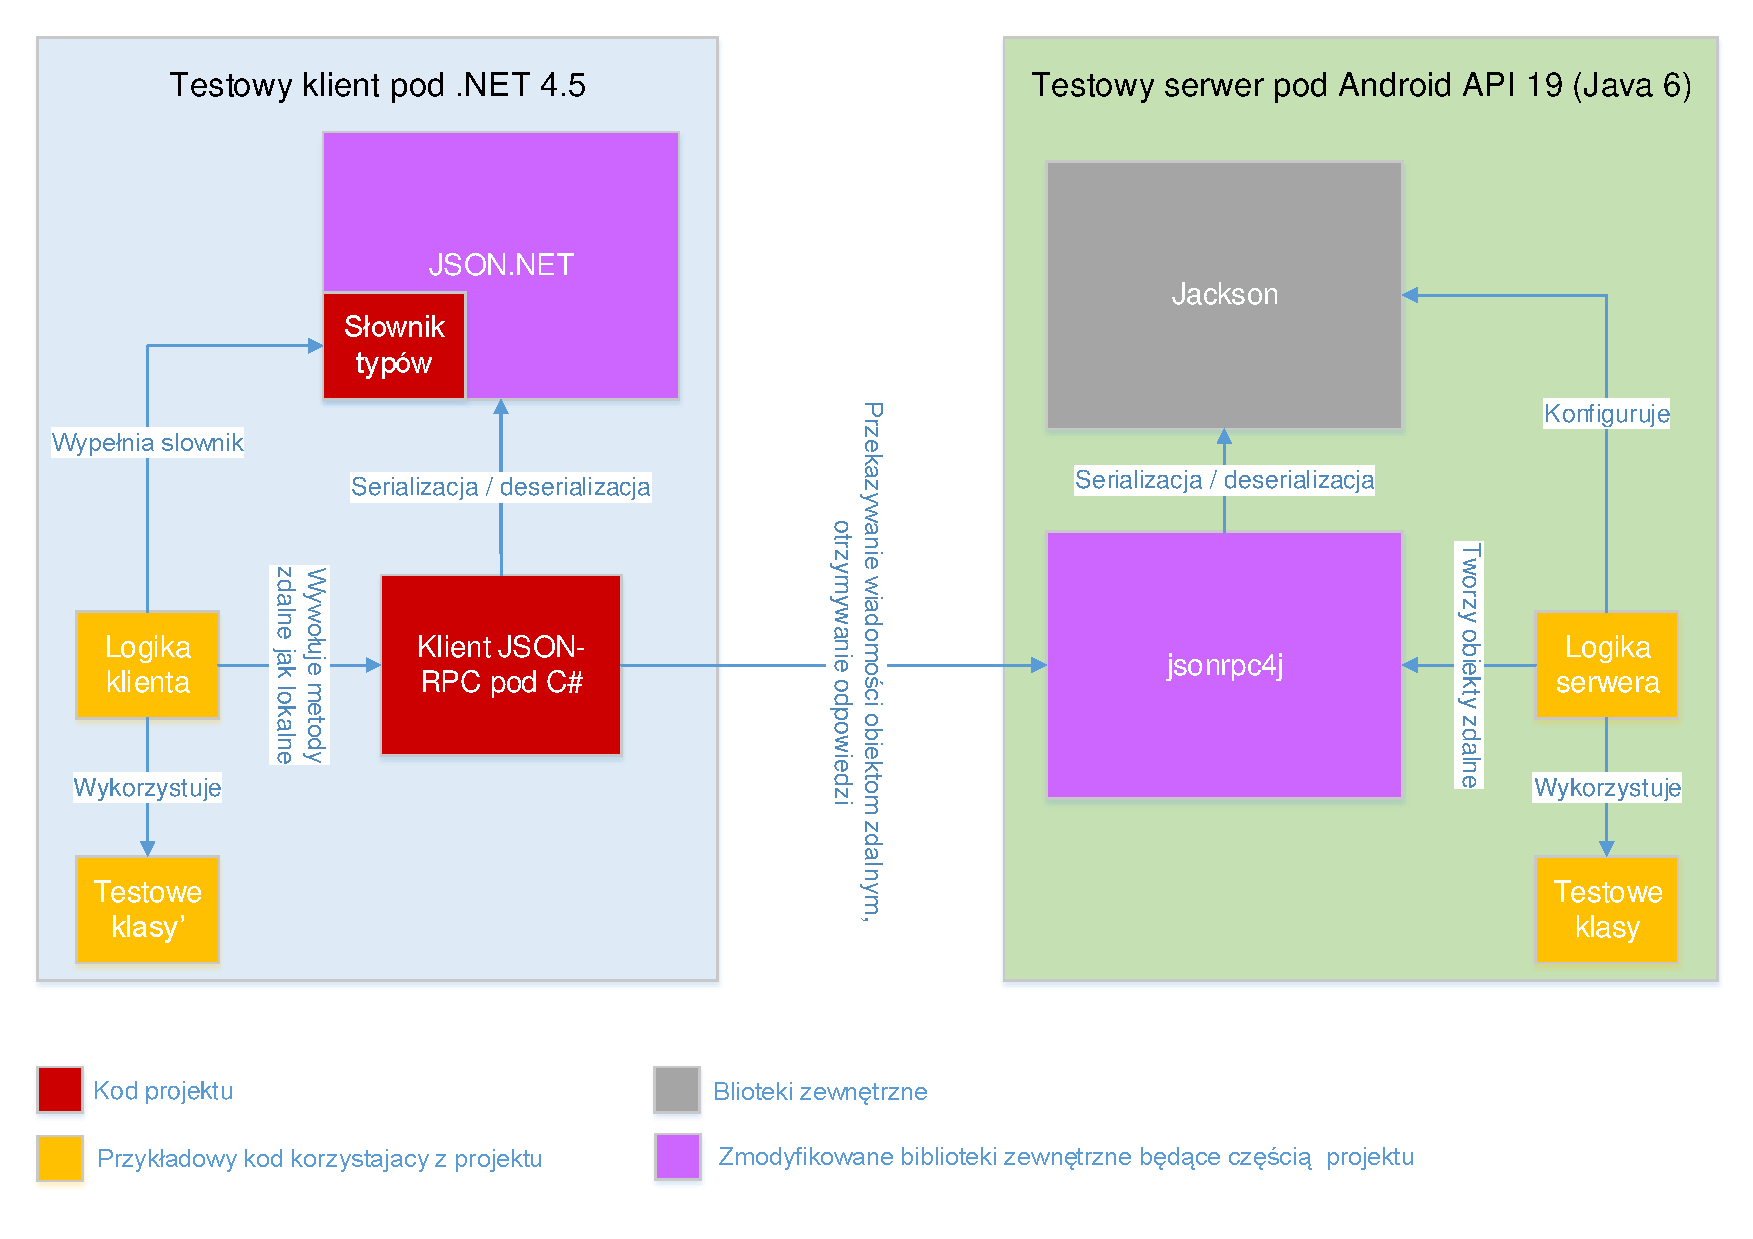
\includegraphics[width=\textwidth]{img/schematy/schemat-implementacji.pdf}
	\caption{Struktura częściowej implementacji projektu.}
	\label{fig:implementation-overview}
\end{figure}

\begin{figure}
	\centering
		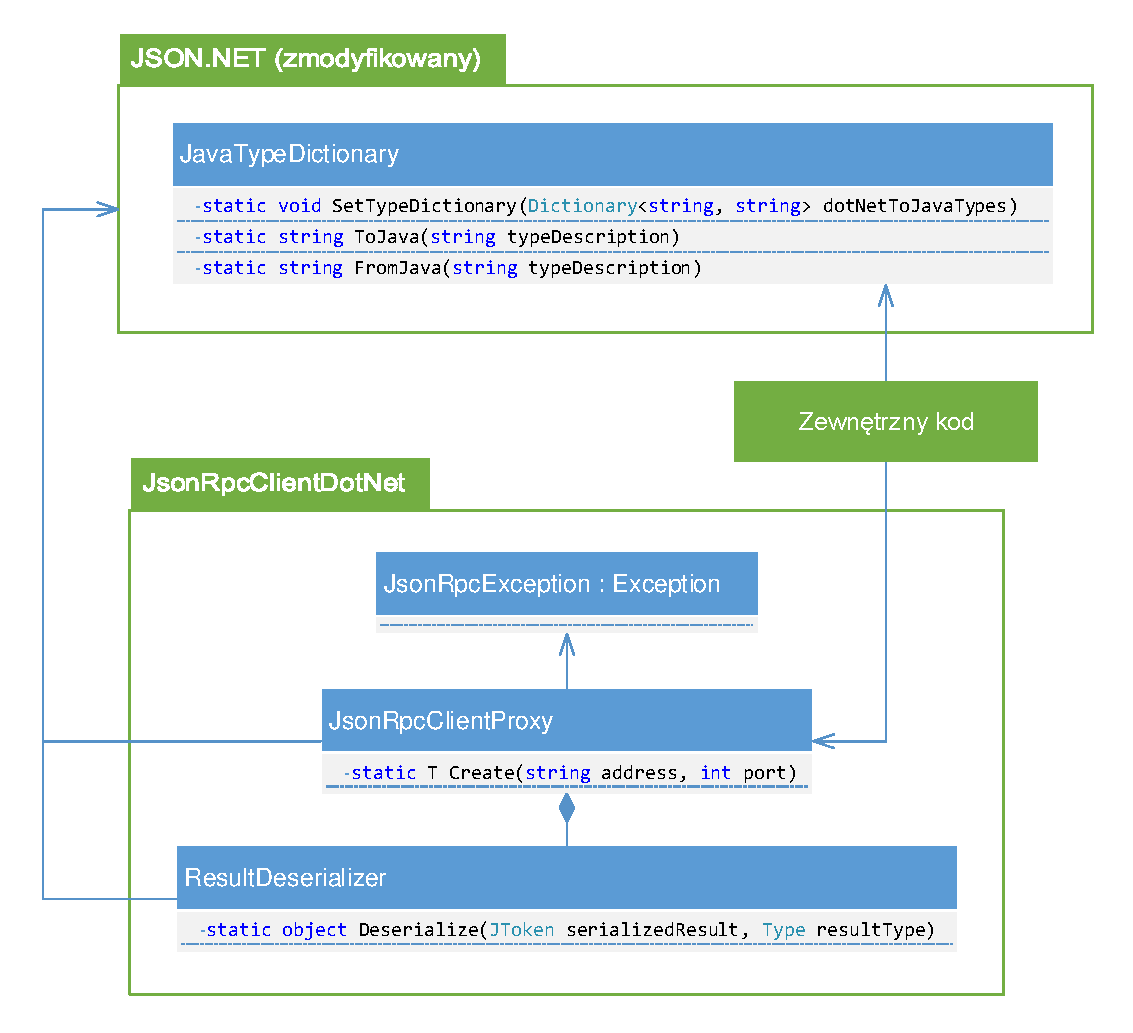
\includegraphics[width=\textwidth]{img/schematy/schemat-klas-net.pdf}
	\caption{Klasy klienta JSON-RPC pod .NET.}
	\label{fig:dot-net-classes}
\end{figure}

\begin{figure}
	\centering
		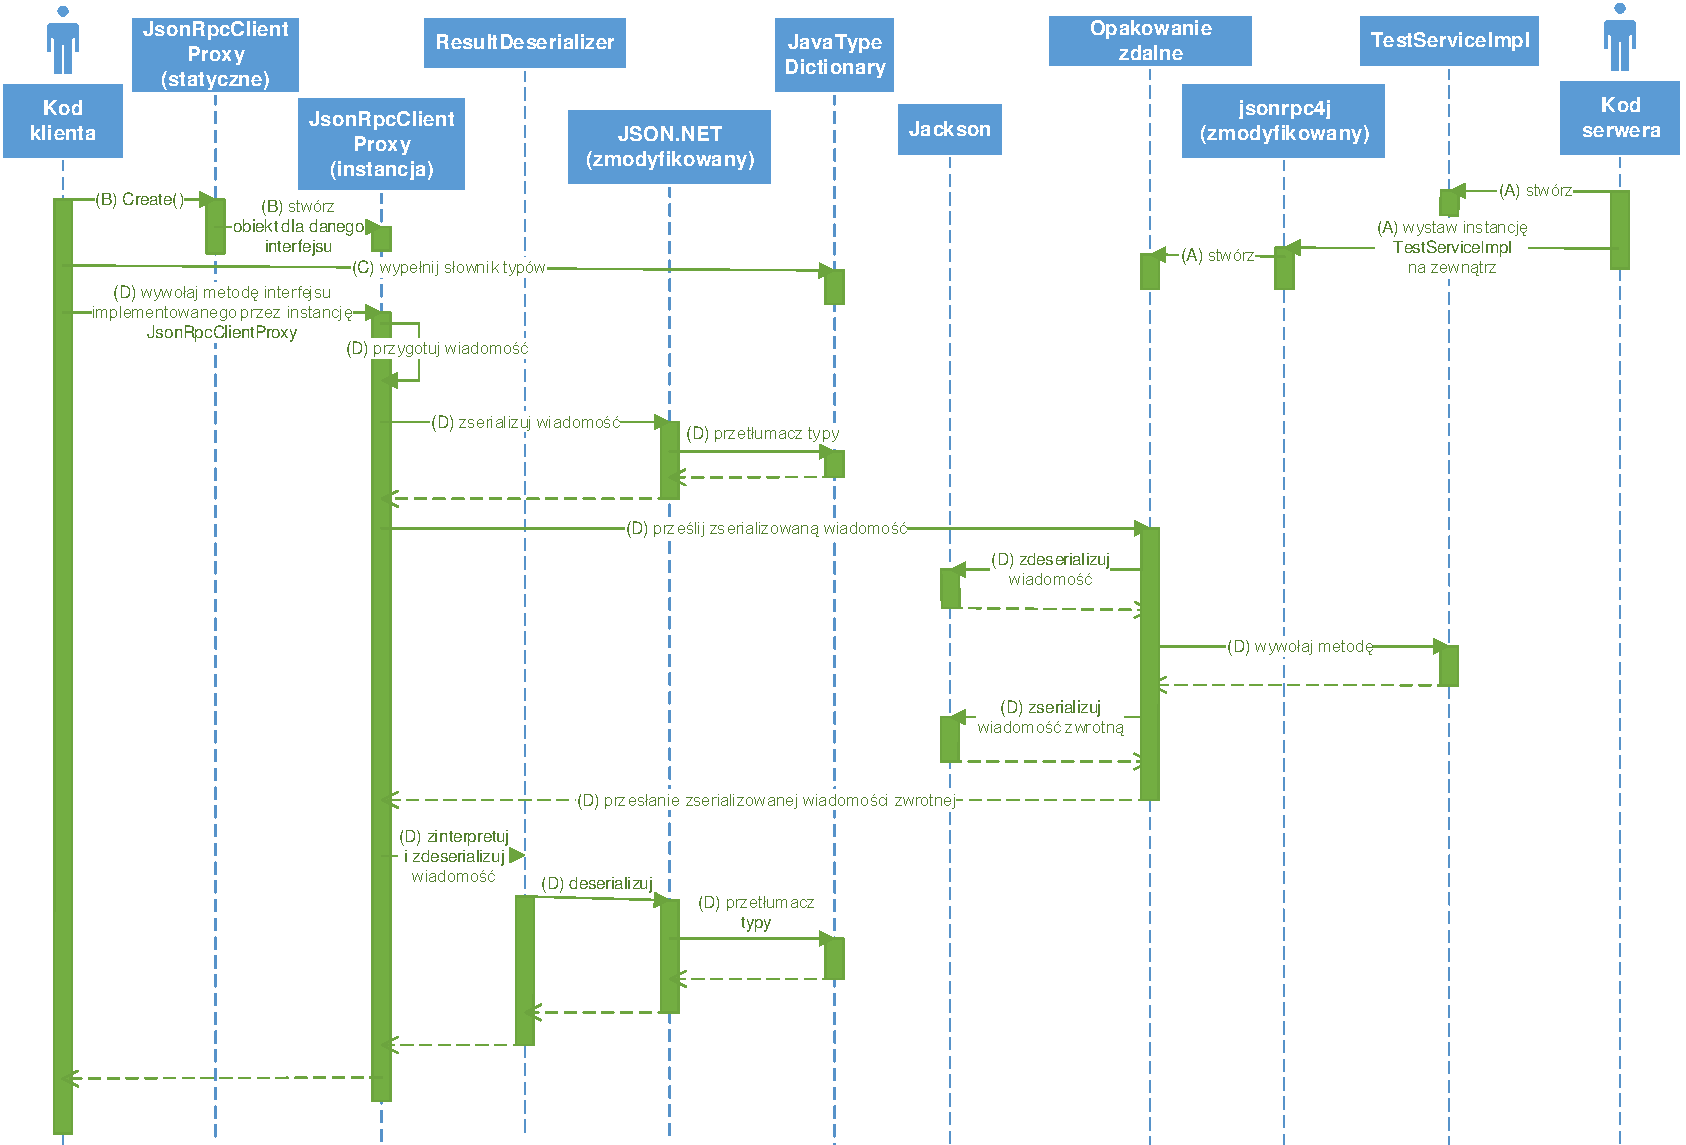
\includegraphics[angle=90,origin=c,scale=0.8]{img/schematy/diagram-sekwencji.pdf}
	\caption[Diagram sekwencji systemu.]{Diagram sekwencji systemu. Są 4 niezależne scenariusze: A, B, C i D. D musi wystąpić po 3 poprzednich.}
	\label{fig:sequence-diagram}
\end{figure}

Sekwencja A to stworzenie obiektu zdalnego. Wyjaśnienie jej kroków:
\begin{itemize}
	\item Kod serwerowy tworzy instancję wybranej klasy, na diagramie jest to \texttt{TestServiceImpl}.
	\item Kod serwerowy wystawia publiczne metody stworzonej instancji \texttt{TestServiceImpl} ,,na zewnątrz'' przy użyciu API jsonrpc4j.
	\item jsonrpc4j tworzy obiekt opakowujący instancję \texttt{TestServiceImpl}; ten obiekt będzie odpowiedzialny za~wołanie metod instancji \texttt{TestServiceImpl} w~odpowiedzi na otrzymywanie wiadomości od klientów JSON-RPC.
\end{itemize}

Sekwencja B -- stworzenie obiektu klienckiego. Faktycznie niezależna od sekwencji A, ponieważ obiekt zdalny musi istnieć dopiero przy pierwszym wywołaniu metody, nie przy stworzeniu obiektu klienckiego. Kroki:
\begin{itemize}
	\item Kod kliencki tworzy instancję obiektu klienckiego (proxy) dla obiektu zdalnego.
	\item Statyczna metoda \texttt{JsonRpcClientProxy} tworzy instancję swojej klasy. Instancja tworzona jest na bazie zadanego interfejsu (np. \texttt{TestService}) i~jest wiązany z~adresem konkretnego obiektu zdalnego.
\end{itemize}

Sekwencja C -- wypełnienie słownika typów. Potrzebne jeśli użytkownik zamierza korzystać z~polimorfizmu parametrów metod zdalnych. Polega na uruchomieniu jednej metody statycznej zmodyfikowanego przeze mnie JSON.NET\footnote{Biblioteka serializacyjna pod .NET; format danych to JSON.}. Wypełniony słownik będzie wykorzystywany do mapowania typów pomiędzy Javą a~.NET przy serializacji i~deserializacji.

Sekwencja D -- wywołanie polimorficznej metody zdalnej, czyli zasadnicza funkcjonalność systemu:
\begin{itemize}
	\item Kod kliencki wywołuję metodę .NETowej wersji interfejsu \texttt{TestService} na instancji \texttt{JsonRpcClientProxy}.
	\item \texttt{JsonRpcClientProxy} przygotowuje wiadomość dla serwera JSON-RPC i~zawiera w~niej przekazane argumenty metody zdalnej.
	\item Wiadomość jest przekazana do serializacji do zmodyfikowanego JSON.NET.
	\item Jeśli zachodzi taka potrzeba, JSON.NET pyta \texttt{JavaTypeDictionary} o~nazwy typów w~Javie, które odpowiadają typom parametrów przekazanych do \texttt{JsonRpcClientProxy}.
	\item \texttt{JsonRpcClientProxy} wysyła zserializawoną wiadomość do serwera JSON-RPC opakowującego instancję obiektu zdalnego.
	\item Po odebraniu wiadomości zakodowanej w~JSON, opakowanie obiektu zdalnego przekazuje ją do deserializacji do Jacksona.
	\item Opakowanie obiektu zdalnego przekazuje zdeserializowane parametry do odpowiedniej metody obiektu zdalnego. On wykonuje te metodę lokalnie i~zwraca otrzymaną wartość do obiektu opakowującego.
	\item Obiekt opakowujący przygotowuje zwrotną wiadomość JSON-RPC umieszczając w~niej obiekt zwrócony z~metody zdalnej. Następnie wiadomość jest serializowana przy użyciu Jacksona.
	\item Zserializowana wiadomość jest zwrócona do \texttt{JsonRpcClientProxy}.
	\item \texttt{JsonRpcClientProxy} przekazuje wiadomość do wewnętrznego obiektu \texttt{ResultDeserializer}. \texttt{ResultDeserializer} rozpoznaje, czy zwrócona wartość to wynik metody czy wyjątek.
	\item \texttt{ResultDeserializer} deserializuje zwróconą wartość wyciągniętą z~wiadomości przy użyciu JSON.NET.
	\item JSON.NET prosi \texttt{JavaTypeDictionary} o~przetłumaczenie nazw typów Javy na odpowiadające nazwy w~.NET.
	\item \texttt{JsonRpcClientProxy} przekazuje do kodu klienckiego przetłumaczony obiekt otrzymany z~metody zdalnej.
\end{itemize}



%Co to? Jakie wymagania spełnia? Co by wchodziło w tego skład lub ogólny sposob realizacji? Realizacja prototypu. Ograniczenia?
\section{Polimorfizm a wspólny format informacji o typach}

\subsection{Wprowadzenie}

\subsubsection{Zdalne metody bez polimorfizmu}
Obie części systemu -- klient (.NET) i~serwer (Android) -- muszą mieć wspólny system oznaczania typów aby wymieniane obiekty mogły być polimorficzne. 
Wspólny format oznaczeń nie jest potrzebny, kiedy nie zależy nam na polimorfizmie, czyli w~większości przypadków wykorzystania zdalnego wywoływania metod (kodu).

Zanim przejdę do przykładów wprowadźmy trochę pseudokodu bazowanego na Javie. Będzie to interfejs obiektu zdalnego, klasa go implementująca oraz klasa danych używana wykorzystywana w~interfejsie; wszystkie znajdujące się w~jednej przestrzeni nazw (\emph{package}). Kod ten znajduje się we fragmencie~\ref{kod:example-remote-classes}.

\begin{lstlisting}[float, frame=single, caption={Przykładowy kod metody zdalnej.}, label=kod:example-remote-classes]
package org.example.test;

public class DataA
{
    public int number;
    public String text;
}

public interface TestService
{        
    DataA modifyData(DataA data);
}

public class TestServiceImpl
{
    DataA modifyData(DataA data)
    {
        data.number += 1;
        data.text += " something added";
        return data;
    }
}
\end{lstlisting}

Załóżmy, że będziemy wywołać metody przy pomocy JSON-RPC. Klasyczne JSON-RPC nie koduje w~żaden sposób informacji o typach. Można by z~.NET przekazać zakodowaną wiadomość, wyglądającą mniej więcej tak:
\begin{lstlisting}[frame=single]
{
    "obiekt": "TestServiceImpl1",
    "metoda": "modifyData",
    "parametry": [
        {
            "number": 13,
            "text": "przykladowy tekst"
        }
    ]
}
\end{lstlisting}
i Java potrafiłaby ją rozkodować. To dlatego, że w~wybranym obiekcie (o~identyfikatorze \texttt{TestServiceImpl1}) istnieje metoda o~nazwie \texttt{modifyData}. Co więcej, przyjmowany przez nią parametr ma dwa obiekty składowe: \texttt{number} i \texttt{text} -- tak samo jak obiekt \texttt{DataA}; dlatego parametr z~JSONa może być zinterpretowany jako \texttt{DataA}\footnote{Zgodnie z~zasadą \emph{Duck Typing}}.

Gdyby obiekt zdalny był klasyczną, a~więc korzystającą z~SOAP, usługą sieciową (\emph{web service}), to powyższy przypadek nie działałby ,,tak po prostu''.
To dlatego, że we wiadomościach SOAP każdy obiekt danych musi być oznaczonym konkretnym typem XML Schema.
Jest to poważny wysiłek, którego w~powyższym przypadku ani serwer, ani klient nie muszą podejmować.

\subsubsection{Zapotrzebowanie na polimorfizm}
\label{need-for-polymorphism}
Póki co, kodowanie informacji o~typach nie jest do niczego potrzebne. Wprowadźmy teraz nową klasę, która dziedziczy po \texttt{DataA}:
\begin{lstlisting}[frame=single]
package org.example.test;

public class DataB extends DataA
{
    public double floatNumber;
}
\end{lstlisting}
Zakładamy też, że po stronie .NET znajduje się odpowiednik zarówno \texttt{DataA}, jak i~dziedziczącej po nim \texttt{DataB}. Także relacja dziedziczenia jest zachowana pomiędzy odpowiednikami. Nazwijmy te odpowiedniki \texttt{DataA'} i~\texttt{DataB'}.

Powiedzmy, że teraz klient chce wywołać metodę \texttt{modifyData} przekazując jako parametr \texttt{DataB'}, a~nie \texttt{DataA'} (które było interpretowane przez serwer jako \texttt{DataA}), jak poprzednim razem.
W~programowaniu obiektowym nie jest to nic dziwnego -- polimorfizm powinien zapewniać to, że obiekt dziedziczący może być zinterpretowany jako bazowy.
Wynikająca z~takiego wywołania wiadomość może wyglądać następująco:
\begin{lstlisting}[frame=single]
{
    "obiekt": "TestServiceImpl1",
    "metoda": "modifyData",
    "parametry": [
        {
            "number": 13,
            "text": "przykladowy tekst",
            "floatNumber": 5.25
        }
    ]
}
\end{lstlisting}

Wiadomość ta różni się od poprzedniej tylko polem \texttt{floatNumber}. W~tej sytuacji serwer może się zachować dwojako, w~zależności od konfiguracji.
Może stwierdzić, że nie ma metody \texttt{modifyData} przyjmującej jeden parametr, który posiada trzy pola: \texttt{number}, \texttt{text} i~\texttt{floatNumber}. W~tej sytuacji nie zostanie wywołana żadna metoda zdalna, a~serwer powinien zwrócić klientowi wyjątek.
Drugim wyjściem jest pominięcie nierozpoznanego przez serwer \texttt{floatNumber} i~zinterpretowanie reszty pól jako obiektu \texttt{DataA}.
Metoda wykona się poprawnie, ale może być to działanie niepożądane przez programistę. Przekazując metodzie instancję \texttt{DataB'} mógł chcieć, żeby obiekt zdalny użył faktycznie jej\footnote{Nie jest, oczywiście, możliwe użycie tej samej instancji obiektu, którą przekazał klient. Chodzi o~dokładną kopię.}. Gdyby działanie metody zależało od typu jej parametru, np. kiedy dokonywana jest inspekcja parametru przy użyciu refleksji, to metoda nie zadziałałaby tak, jak oczekiwał tego programista.

Oczywista jest przydatność polimorfizmu gdyby na przyjmowanym parametrze była wywoływana jakaś metoda. Jest to standardowy sposób rozszerzania działania kodu bez jego przepisywania, stosowany w~programowaniu obiektowym.
Klasy, które tutaj nazywam ,,klasami danych'' i~używam jako argumentów dla metod zdalnych mogą mieć metody, jednak wprowadza to problem przy utrzymywaniu bliźniaczych klas we dwóch językach.

Łatwo jest przepisać na inny język klasę, które posiada tylko pola i~żadnych metod -- może to często zrobić nawet automat.
Metody, natomiast, mogą być wyzwaniem nawet dla człowieka. Nawet, jeśli mowa o~prostej logice, to utrzymanie równoznaczności metod w~obu językach może być wymagające.
Co prawda, równoznaczność nie jest wcale niezbędna. Po obu stronach barykady klasa może mieć zupełnie inne metody i~zachowanie, zachowując te same pola. Ma to jednak wyraźnie zły wpływ na przejrzystość kodu całego systemu.

Aby obronić polimorfizm w~obiektach zdalnych, mogę dać nieco wydumany przykład metody, która rysuje koła, a~jest sparametryzowana obiektem typu \texttt{Object} (czyli dowolnym). Domyślnie rysuje ona jedno koło o promieniu 5.0, ale w~przekazanym obiekcie szuka pól int (pierwsze zamienia na ilość kół) i double (pierwszego double zamienia na promień rysowanych kół) wyciąga pola przekazanego obiektu.
Inspekcja obiektów może być używana chociażby przy różnego rodzaju konfiguracjach. Np.\ każdy obiekt hipotetycznego typu \texttt{AdresBazyDanych} znajdujący się w~przychodzących do metod zdalnych parametrach ma zostać podmieniony na wartość pożądaną przez serwer. Kiedy dalej obiekt zdalny będzie wykonywać jakieś operacje na przesłanych parametrach to będzie używany adres skonfigurowany na serwerze, a~nie jakiś nieznany przysłany z~zewnątrz.
Mniej więcej tak dzieje się w~Spring IoC\footnote{\url{http://docs.spring.io/spring-framework/docs/current/spring-framework-reference/html/beans.html}} -- kontenerze odpowiedzialnym za automatyczną konfigurację aplikacje webowej opartej na frameworku Spring.

%Aby programista nie tracił niespodziewanie żadnych danych i miał po drugiej stronie to, czego chce
%Aby sytuacja była jasna typy muszą być oznaczane. Do tego, oznaczanie typów musi być jednolite. Musi być słownik itp. Wtedy wiadomość wyglądałaby tak, bo klient by sobie przetłumaczył typy (zakładamy, że robi to klient). Serwer by sobie odebrał i byłoby git.
%


\subsection{Plan rozwiązania}
W~ogólności -- aby polimorfizm metod zdalnych był możliwy potrzeba aby klient i~serwer:
\begin{itemize}
	\item oznaczały typy obiektów, kiedy nie są one jednoznaczne;
	\item oznaczały typy w~sposób zrozumiały dla drugiej strony;
	\item miały dostęp do typów odpowiadającym typom przesyłanym z~drugiej strony (typy lustrzane).
\end{itemize}

O~lustrzanych typach pisałem już we wprowadzeniu powyżej. Przykładowy program w~Javie posiadał typy \texttt{DataA} i~\texttt{DataB} po nim dziedziczący. Kod pod .NET posiadał, natomiast, odpowiadające im \texttt{DataA'} i~\texttt{DataB'}.
Zakładając, że używanym przez nas językiem platformy .NET będzie C\#, klasy te powinny wyglądać tak:
\begin{lstlisting}[frame=single]
namespace SerializationTest
{
  public class DataA
  {
      public int number;
      public string text;
  }
  
  public class DataB : DataA
  {
      public double floatNumber;
  }
}
\end{lstlisting}
W tym przypadku Java i~C\# są do siebie bardzo zbliżone.

Można zauważyć kilka rzeczy:
\begin{itemize}
	\item Nazwy klas nie zawierają prim (') -- będą używane tylko w~skróconych oznaczeniach w~tekście.
	\item Nazwa paczki Javy (\texttt{org.example.test}) i~przestrzeń nazw z~.NET (\texttt{SerializationTest}) nie są takie same; pełne nazwy klas będą następujące: \texttt{org.example.test.DataA} i~\texttt{org.example.test.DataB} (Java), \texttt{SerializationTest.DataA} i~\texttt{SerializationTest.DataB} (.NET).
	\item Klasy z~C\# zachowują zależność dziedziczenia.
	\item Odpowiadające sobie klasy mają taki sam zestaw publicznych pól; ważny jest ich typ i nazwy, nie jest ważna kolejność.
	\item Mimo tego, że tutaj odpowiadające sobie klasy mają takie same nazwy, to nie jest to potrzebne (choć zapewnia czytelność).
	\item Aby logicznie powiązać odpowiadające sobie klasy musi istnieć pewnego rodzaju słownik; to on pokaże, że np. \texttt{org.example.test.DataA} jest odpowiednikiem \texttt{SerializationTest.DataA}; zależność ta jest wzajemna.
\end{itemize}

%Oznaczanie typów wymaga słownika. Można by wymusić takie same namespace'y i package, ale każde mają inne zasady nazewnictwa. Można by też wprowadzić identyfikacje po ostatnim członie, ale wtedy stracilibyśmy korzyść z osobnych przestrzeni nazw.

Odpowiadające sobie typy danych w~językach tak podobnych jak Java i~C\# mogłyby teoretycznie być uzyskiwane przez automatyczne tłumaczenie -- z~Javy do .NET lub odwrotnie.
Nie udało mi się jednak uruchomić żadnego narzędzia, które powinno to potrafić.

Oznaczenie typów może polegać na dodawaniu do obiektu specjalnego pola. W~poniższym przykładzie, przedstawiającym hipotetyczną wiadomość wysłaną z~.NET, to pole zostało nazwane \texttt{\$typ} i~posiada wartość typu \emph{string} zawierającą pełną, jednoznaczną nazwę typu.
\begin{lstlisting}[frame=single]
{
    "obiekt": "TestServiceImpl1",
    "metoda": "modifyData",
    "parametry": [
        {
            "$typ": "SerializationTest.DataB"
            "number": 13,
            "text": "przykladowy tekst",
            "floatNumber": 5.25
        }
    ]
}
\end{lstlisting}

Po dodaniu takiego pola serwer powinien wiedzieć jaki konkretnie obiekt otrzymał.
Gdyby przekazano obiekt \texttt{DataA} to informacja o~typie (pole \$typ) nie byłaby potrzebna, ponieważ \texttt{DataA} jest spodziewanym typem parametru metody \texttt{modifyData}.


\subsection{Implementacja}
\subsubsection{Założenia}
Od razu zakładam, że serializacja danych będzie oparta o~JSON a~protokołem komunikacyjnym będzie JSON-RPC. Pozwoli to na lekką komunikację i~stosunkowo prostą implementację.
Ponadto, biblioteka JSON-RPC dla języka Java -- jsonrpc4j\footnote{Patrz punkt~\ref{jsonrpc4j}.}, może po modyfikacji działać na Androidzie.
Po stronie .NET posłużę się otwartą biblioteką do serializacji do JSON -- JSON.NET.

Jackson jest biblioteką serializacyjną z~której korzysta jsonrpc4j. Zarówno Jackson jak i~JSON.NET mają dużo możliwości konfiguracji. Obie posiadają też możliwość kodowania (przez specjalne pola) informacji o typach.

\subsubsection{Porównanie działania Jackson i~JSON.NET}
Zestawienie ich działania dla kilku przypadków znajduje się we fragmentach \ref{kod:serilization-objects}, \ref{kod:serialization-arrays}, \ref{kod:serialization-lists}, \ref{kod:serialization-dicts}. Różnice stylu oznaczania typów są w~tabeli~\ref{tab:jackson-jsonnet-differences}

\begin{lstlisting}[float, frame=single, caption={Porównanie serializacji obiektów typu \texttt{DataA}}, label=kod:serilization-objects]
\\ Jackson
{
    "@class":"org.example.test.DataA",
    "numberA":13,
    "text": "przykladowy tekst"
}

\\JSON.NET
{
    "$type": "SerializationTest.DataA, TestDataLib",
    "number": 13,
    "text": "przykladowy tekst"
}
\end{lstlisting}

\begin{lstlisting}[float, frame=single, caption={Porównanie serializacji tablicy obiektów typu \texttt{Object}. Tablica zawiera wartość typu \texttt{int} oraz wartość typu \texttt{string}}., label=kod:serialization-arrays]
\\ Jackson
[
  "[Ljava.lang.Object;",
  [
    28,
    "jakis tekst"
  ]
]

\\ JSON.NET
{
  "$type": "System.Object[], mscorlib",
  "$values": [
    28,
    "jakis tekst"
  ]
}
\end{lstlisting}

\begin{lstlisting}[float, frame=single, caption={Porównanie serializacji listy obiektów typu \texttt{Object}. Lista zawiera wartość typu \texttt{int} oraz wartość typu \texttt{string}}., label=kod:serialization-lists]
\\ Jackson
[
  "java.util.ArrayList",
  [
    28,
    "jakis tekst"
  ]
]

\\ JSON.NET
{
  "$type": "System.Collections.Generic.List`1[[System.Object, mscorlib]], mscorlib",
  "$values": [
    28,
    "jakis tekst"
  ]
}
\end{lstlisting}

\begin{lstlisting}[float, frame=single, caption={Porównanie serializacji słownika/mapy (\emph{dictionary/map}) mapującego wartość typu \texttt{string} do wartości typu \texttt{int} (\texttt{int} jest kluczem).}, label=kod:serialization-dicts]
\\ Jackson
{
  "@class":"java.util.HashMap",
  "1":"pierwszy",
  "2":"drugi",
  "3":"trzeci"
}

\\ JSON.NET
{
  "$type": "System.Collections.Generic.Dictionary`2[[System.Int32, mscorlib],[System.String, mscorlib]], mscorlib",
  "1": "pierwszy",
  "2": "drugi",
  "3": "trzeci"
}
\end{lstlisting}

\begin{table}[htbp]              
	\centering
		\begin{tabular}{ | p{0.25\textwidth} || p{0.30\textwidth} | p{0.35\textwidth} | }
			\hline
				& \textbf{Jackson} & \textbf{JSON.NET} \\
				\hline \hline
				Nazwa pola specjalnego pola zawierającego oznaczenie typu & \texttt{@class} & \texttt{\$type}. \\
				\hline
				Oznaczenie typu zawiera & Pełną nazwę klasy & Pełną nazwę klasy oraz nazwę źródłowej biblioteki (DLL). \\
				\hline
				Oznaczenie typu list i~tablic & Opakowanie w~dodatkową listę, której pierwszym elementem jest \texttt{string} z~nazwą typu, a~drugim oryginalna kolekcja. & Opakowanie w~obiekt z~dwoma polami: \texttt{\$type} i~\texttt{\$values} zawierające oryginalną kolekcję. \\
				\hline
				Oznaczenie typów generycznych & Nie ma i~nie jest możliwe ze względu na \emph{,,type erasure''}. & Oznaczane przy użyciu składni <nazwa-typu-generycznego>`<ilość-parametrów-typu>[[<nazwa-typu-1>], [<nazwa-typu-2>], ...] \\
				\hline
		\end{tabular}
	\caption{Różnice w~stylu oznaczania typów pomiędzy Jackson a JSON.NET.}
	\label{tab:jackson-jsonnet-differences}
\end{table}

\subsubsection{Dookreślenie planu rozwiązania}
Mimo, że JSON.NET posiada duże możliwości konfiguracji stylu serializacji, zdecydowałem się na modyfikację jego źródeł, zamiast pisania biblioteki na nim bazującej. Nie wszystko da się zrobić przez konfigurację, np.\ nie da się zmienić nazwy specjalnego pola z~typem (\texttt{\$type}).
Wydaje się też, że zbudowanie programu imitującego sposób serializacji Jacksona korzystającego z~JSON.NET byłoby znacznie bardziej pracochłonne niż przerobienie JSON.NET, aby robił to samo.

Zmodyfikowany JSON.NET traci zgodność ze swoim niezmodyfikowanym odpowiednikiem.
Przestają też działać niektóre zaawansowane funkcje, np. zapisywanie referencji do obiektów znajdujących się w~pamięci.
Można je pominąć, ponieważ nie są przydatne w~moim zastosowaniu, tj.\ w~serializacji obiektów danych, które mają być wysyłane na inną platformę.

Aby JSON.NET miał wspólny z~Jackson format informacji o~typach trzeba:
\begin{itemize}
	\item zmienić nazwę pola oznaczającego typ z~\texttt{\$type} na @class;
	\item zmienić sposób serializacji tablic i~list na taki, który imituje Jacksona;
	\item zmienić sposób deserializacji tablic i~list, aby mogły być przyjmowane od Jacksona;
	\item utrzymywać po obu stronach (Java, C\#) odpowiadające sobie klasy danych;
	\item stworzyć słownik łączący pełne nazwy klas w~Javie z~odpowiednikami w~.NET i~vice versa.
\end{itemize}

Brak informacji o~konkretnym typie typów generycznych zserializowanych Jacksonem będzie problemem, jeśli po drugiej stronie typ ten nie będzie mógł być jednoznacznie wywnioskowany. Np.\ kiedy nie ma żadnych założeń co do typu obiektu -- będzie to typ dziedziczący po \texttt{Object}.
Powiedzmy, że zserializowano obiekt, którego jedno pole ma typ generyczny, np.\ jako pole typu \texttt{ArrayList<String>}. W~takim przypadku konkretny typ szablonu \texttt{ArrayList} będzie mógł być wywnioskowany i~system będzie działał dobrze.
Ogólnie -- wrodzoną wadą systemu będzie to, że typy generyczne nie zawsze będą działać.
Nie jest to winą Jacksona, a~mechanizmu języka Java zwanego \emph{,,type erasure''} usuwającego informacje o~faktycznym typie typu generycznego w~trakcie wykonywania kodu.

Jackson nie obsługuje też informacji o bibliotece. Schemat nazywania pakietów w~Javie powinien, jednak, zapewniać ich unikalność, więc brak nazwy biblioteki to nie problem.

\subsubsection{Ostateczny kształt rozwiązania}
JSON.NET ma 14401 linii kodu, używany przeze mnie podzbiór Jackson -- 63497. Obie biblioteki są dobrze napisane i~konfigurowalne, ale nie zakładają dużej ingerencji w~system oznaczania typów, który to w~obu przypadkach jest inny i~specyficzny.
W~przypadku JSON.NET, który próbowałem zmodyfikować mechanizmy wykrywania i~oznaczania typów są dość mocno uwiązane z~resztą biblioteki. Z~racji natury procesów serializacji i~deserializacji kod jest rekurencyjny i~mocno rozgałęziony.

Przez to nie udało się dopasować serializacji tablic i~list do formatu Jacksona. Zdecydowanie nie jest to niemożliwe, ale wysiłek do tego potrzebny nie zmieścił się w~ramach tej pracy. 

Całkowicie, natomiast udała się serializacja dowolnych pojedynczych (nawet skomplikowanych) obiektów. Dzięki temu można uzyskać sprawne polimorficzne metody zdalne.

Wykonane modyfikacje JSON.NET według klas:
\begin{description}
\itemtitle{\texttt{JavaTypeDictionary}}
Nowa klasa statyczna. Można ją zainicjować przy pomocy słownika, czyli obiektu typu \texttt{Dictionary}. Klasa go zapamiętuje oraz tworzy słownik odwrotny (klucze i~wartości zamienione rolami) dla szybszego przeszukiwania. Klasa ta będzie używana przez resztę JSON.NET do tłumaczenia nazw typów.

\itemtitle{\texttt{JsonSerializerInternalWriter}}
W~metodzie \texttt{WriteTypeProperty} dodano tłumaczenie zapisywanych nazw typów na odpowiedniki z~Javy.

\itemtitle{\texttt{JsonTypeReflector}}
Stała \texttt{TypePropertyName} zmieniona z~\texttt{\$type} na \texttt{@class} aby zapewnić zgodność z~Jacksonem. JSON.NET rozpoznaje specjalne pola obiektów po tym, że zaczynają się od ,,\$''. Dlatego ta zmiana psuje zgodność z~oryginalnym JSON.NET.

\itemtitle{\texttt{JsonSerializerInternalReader}}
Metoda \texttt{ReadMetadataProperties} stosowała wspomniany wcześniej mechanizm wykrywania specjalnych pól obiektów polegający na sprawdzaniu, czy  pierwszy znak nazwy to ,,\$''. Został on zamieniony na ,,@'' aby mogło być wyłapane pole \texttt{@class}. Ponadto, metoda \texttt{ResolveTypeName} korzysta z~\texttt{JavaTypeDictionary} do tłumaczenia nazw klas z~Javy na .NET.

\end{description}

%Żeby słownik był dobry dla programisty, to dobrze jakby
%Potrzebny jest system mapujący nazwy typów w jednym środowisku, na nazwy z drugiego. Mógłby działać na zasadzie słowników. Żeby zmniejszyć nakład pracy mogły by one być generowane automatycznie zgodnie z jakąś zasadą.
%Pewnie potrzebny by był też system ładowania klas.
%Może jakiś schemacik tego ładowania i jakby mapowanie działało przy serializacji, deserializacji.

%Potrzebny byłby system ładowania bibliotek i klas z nich. Ale i tak nie dostarczam gotowego systemu, tylko taki prototyp, wiec chyba mogę to pominąć. Tłumaczenia klas też nie będzie. Albo tłumaczenie mogę pominąć, ładowanie zrobić konfigurowane, tj. tak jak słownik typów byłby spis bibliotek (np. z ich pełnymi ścieżkami). Te biblioteki byłyby ładowane do Assembly w .NET i do aktualnego class loadera w javie. Można by to prosto obtestować.



\section{Zdalne wywoływanie metod na Androidzie}
\label{android-rpc}

\subsection{Wybrana forma zdalnego wywoływania metod}
Jako format zdalnego wywoływania metod w~moim systemie wybrałem JSON-RPC 2.0. Przez swoją prostotę zyskuje on odporność na błędy i~łatwość implementacji.
Poza tym spełnia wszystkie moje wymagania -- identyfikuje docelowe obiekty i~metody oraz pozwala rozszerzać sposób serializacji parametrów metod.
Każda wiadomość posiada też identyfikator, który wspomaga rozumienie serii wiadomości w~wymianie między klientem a serwerem jako logicznej ,,rozmowy''.

Ponadto od wersji 2.0, JSON-RPC posiada mechanizm rozszerzania swoich wiadomości (\emph{Extensions})~\cite{json-rpc-extensions}.
Dzięki tym rozszerzeniom można by wyróżnić pewne szczególne wiadomości dla serwera, np.\ takie, które mają wywołać stworzenie nowej instancji zdalnego obiektu lub usunięcie starej.
Taka funkcjonalność jest zawarta w~zebranych wcześniej wymaganiach systemowych, jednak jako mało kluczowa została poświęcona na rzecz realizacji działającego prototypu.

Jednakże kluczowym elementem, który przyczynił się do decyzji o~użyciu JSON-RPC było istnienie biblioteki jsonrpc4j (opisanej w~punkcie~\ref{jsonrpc4j}). Była prosta w~użyciu, funkcjonalna i~nie brakowało jej dużo, aby mogła działać na Androidzie.


\subsection{Plan rozwiązania}
Gdyby nie skupiać się na polimorfizmie, to, poza zwykłym JSON-RPC, część serwerowa mojego prototypu nie potrzebuje niczego więcej.
Wystarczy stworzyć obiekt posiadający publiczne metody i~wystawić go na zewnątrz przy pomocy klasy \texttt{JsonRpcServer} z~jsonrpc4j.
W~tym momencie dowolny klient JSON-RPC, napisany w~dowolnym języku, może wywoływać kod na serwerze.
Jeśli tym serwerem jest Android, a~tak będzie w~tym przypadku, to klient JSON-RPC może zdalnie wykorzystywać API Androida i~nim zarządzać. A~więc spełnione jest jedno z~wymagań.

Trzeba tylko pamiętać o~posiadaniu po obu stronach wyglądających tak samo typów (wyjaśnione w~punkcie~\ref{need-for-polymorphism}).
Chyba, że wszystkie przyjmowane i~zwracane przez zdalne metody typy są typami prostymi (\texttt{int}, \texttt{double}, \texttt{bool}, też \texttt{string}) -- są one powszechnie dostępne i~rozumiane, więc nie będzie żadnych problemów.

Klasa \texttt{JsonRpcServer} umożliwia przyjmowanie połączeń do obiektu zdalnego na kilka sposobów, jednak wszystkie poza jednym wymagają bibliotek, które nie są dostępne dla Androida, tylko dla standardowej (właściwie nawet rozszerzonej o~Javę EE) Javy.
Sposób, który może działać na Androidzie polega na powiązaniu obiektu z~socketem TCP. Obiekt dostaje jeden port, na którym nasłuchuje wiadomości.
Klienci wysyłają zakodowane JSONem po nawiązaniu połączenia TCP z~konkretnego portem, na konkretnym adresie IP.
Tak że na jednym serwerze może być wystawionych tyle obiektów zdalnych, ile jest portów TCP na wszystkich interfejsach sieciowych hosta.
W~przypadku Androida zazwyczaj jest tylko jeden interfejs, co i~tak daje dziesiątki tysięcy portów.

Trzeba ustawić zgodne polimorficzne serializatory zarówno dla klienta jak i~serwera i~wywołać jakąś z~metod, którymi testowałem polimorfizm w~rozdziale~\ref{similar-technologies}.

Kiedy zaczyna nam zależeć na polimorfizmie metod zdalnych, trzeba zwrócić uwagę na konfigurację serializatorów.
Jackson, który jest biblioteką serializacyjną używaną przez jsonrpc4j ma zdolność oznaczania typów. API jsonrpc4j pozwala, na szczęście, na konfigurację parametrów Jacksona. Czyli możemy sprawić, że serwer będzie zarówno rozumiał oznaczenia typów, jak i~sam będzie je stosował.

Polimorfizm ma swoją cenę -- serwer przestaje być uniwersalnie zgodny z~klientami, ponieważ informacje o~typie we wiadomościach JSON nie są częścią standardu JSON-RPC 2.0.
Aby móc rozmawiać z~serwerem, klient musi teraz mieć tak samo działający serializator.
Jest to proste dla innych aplikacji korzystających z~Jacksona, chociaż ich twórcy musieliby je świadomie skonfigurować. Ale inne biblioteki albo w~ogóle nie potrafią oznaczać typów, albo robią to w~niekompatybilny sposób.
Tak było w~przypadku JSON.NET, którego jednak udało mi się (częściowo) dopasować do Jacksona. 


\subsection{Realizacja}
Przy próbie uruchomienia jsonrpc4j na Androidzie od razu wystąpił błąd. Okazało się, że mimo tego, co jest napisane na stronie projektu\footnote{,,(\ldots)In fact, the client and server both work in an Android environment.(\ldots)~\cite{jsonrpc4j}} nie można uruchomić serwera na Androidzie.
To dlatego, że klasa \texttt{JsonRpcServer} zawiera zależności do bibliotek, które nie są dostępne dla Androida, a~Java musi móc je załadować, kidy ładuje klasę.

Na szczęście można było podzielić klasę na dwie części -- tę podstawową, która umożliwia wystawianie obiektów zdalnych na portach TCP i~tę zaawansowaną, która dziedziczy po podstawowej i~zależy od bibliotek niedostępnych Androidowi.
Wydzieloną klasę bazową nazwałem \texttt{JsonRpcBasicServer}. Aby wystawić zdalny obiekt wystarczy kod przedstawiony we fragmencie~\ref{kod:android-remote-object}.

\begin{lstlisting}[float, frame=single, caption={Tworzenie obiektu zdalnego przy pomocy jsonrpc4j dostosowanego do Androida.}, label=kod:android-remote-object]
TestServiceImpl service = new TestServiceImpl();
JsonRpcBasicServer serverBase = new JsonRpcBasicServer(
    ServerThread.createMapper(),
    service,
    TestService.class);
		
bindAddress = InetAddress.getByName("0.0.0.0");
StreamServer server = new StreamServer(
    serverBase,
    maxThreads,
    port,
    0,
    bindAddress);

server.start();
\end{lstlisting}

Tym samym serwer jest całkowicie sprawny i~umożliwia wystawianie dowolnych metod Javy (poza metodami generycznymi) do konsumpcji dla wszystkich klientów JSON-RPC.
Ponieważ po moich zmianach nie ma żadnego spadku funkcjonalności będę próbował przyłączyć je do oryginalnego projektu.



\section{Klient JSON-RPC pod .NET}
\subsection{Wprowadzenie}
Kod kliencki mojego systemu potrzebuje możliwości wołania serwera JSON-RPC.
Okazuje się, że implementacje w~.NET, np. JSON-RPC.NET (opisane w~punkcie~\ref{json-rpc-net}) nie posiadają takiej możliwości.
Potrafią łatwo wystawiać obiekty zdalne na zewnątrz, ale nie mają właściwie żadnych udogodnień do ich konsumowania.
Istnieją jedynie dyskusje na temat części klienckiej i~dość prymitywne ich implementacje.
Te implementacje i~tak zmuszają do ,,własnoręcznego'' złożenia wiadomości JSONowej\cite{json-rpc-net-client}.

W~przypadku rozwiniętych \emph{frameworków} jak WCF, czy JAX-WS normalne jest, że można w~prostu sposób stworzyć obiekt proxy do serwisu zasilając go jakimś interfejsem.
Następnie obiekt ten może być wołany jak zwykły obiekt lokalny spełniający zadany interfejs.
Taką funkcjonalność posiada też jsonrpc4j.

Postanowiłem stworzyć kod, który pozwoli na eleganckie tworzenie obiektów klienckich i~wywoływanie na nich metod.

\subsection{Realizacja}
Udało mi się stworzyć klienta, który jest bardzo wygodny w~użyciu (fragment~\ref{kod:my-json-rpc-clinet}).
Można go tworzyć i~wykorzystywać jak normalny obiekt. Zwraca też normalne obiekty.
Jeśli połączy się go ze zmodyfikowanym przeze mnie JSON.NET, to potrafi także przekazywać polimorficzne parametry do mojego serwera.

Niestety nie ma jeszcze zaawansowanej logiki odpowiadającej za odporność połączenia, czy ponowne próby wysłania wiadomości. Jeśli coś pójdzie nie tak w~warstwie TCP to zostanie rzucany wyjątek i~wywołanie metody się nie uda.
Nie jest to jednak duża wada.

Też tłumaczenie typów wyjątków nie jest jeszcze wspierane.
To dlatego, że nie są one przekazywane tak, jak normalne obiekty i~wymagają specjalnego sposobu dekodowania (patrz fragment~\ref{kod:json-rpc-exception}).
Jeśli coś pójdzie nie tak w~wykonywaniu zdalnej metody (też nie zostanie ona znaleziona) mój klient rzuca ogólny wyjątek \texttt{JsonRpcException}, który zawiera w~sobie wiadomość i~typ wyjątku rzuconego po drugiej stronie.
Idealnie byłoby, gdyby na bazie wiadomości z~błędem otrzymywanej od serwera klient tworzył odpowiednią instancję wyjątku i~go propagował.

\begin{lstlisting}[float, frame=single, caption={Tworzenie obiektu proxy do obiektu zdalnego przy użyciu mojej implementacji klienta JSON-RPC pod .NET.}, label=kod:my-json-rpc-clinet]
TestService service = JsonRpcClientProxy<TestService>.
      Create(ipAddressOrHostname, port);

DataA parameter = new DataA();
try
{
    DataA returnedObject = service.modifyData(parameter);
}
catch(JsonRpcException ex)
{
    \\ wyswietl tresc wyjatku z serwera
    Console.WriteLine(ex.Message);
}
\end{lstlisting}

\begin{lstlisting}[float, frame=single, caption={Wiadomość od serwera JSON-RPC zawierająca wyjątek.}, label=kod:json-rpc-exception]
{
  "jsonrpc": "2.0",
  "id": 1, "error": {
    "code": 0,
    "message": "Wiadomosc w exceptionie jakas",
    "data": {
      "exceptionTypeName": "java.io.IOException",
      "message": "Wiadomosc w exceptionie jakas"
    }
  }
}
\end{lstlisting}



%\section{Tworzenie zdalnych obiektów na żądanie klienta(TODO)}
%Klient musi mieć specjalną metodę, którą będzie wywoływał stworzenie zdalnego obiektu, któremu dalej będzie wysyłał wywołania.
%Można to zrealizować przy pomocy mechanizmu rozszerzeń (\emph{Extensions}) standardu JSON-RPC 2.0.
%Normalnie tego nie ma, bo raczej mamy dane żyjące serwisy i z nimi gadamy. Też normalnie nie operuje się na typie serwisu. Tu będzie trzeba właśnie podać typ serwisu, jaki chcemy. No w sumie WCF i JAX-WS to jakoś tam robią. Ale one mają jakby serwis i tak wolnostojący i dopiero w nim robią instancje. U mnie będzie jeden główny serwer i pod nim instancje wszystkiego.
%%https://jsonrpcx.org/Main/HomePage
%%http://grokbase.com/t/gg/json-rpc/138ce80p54/what-are-rpc-extensions
%%consolidation service w JSON-RPC?
%
%
%
%\section{Wersja z Thriftem}
%To mogłoby robić prawie wszystko. Działałoby jako niezależny system i nie korzystało z poprzednich komponentów. Nie realizowałoby jednak wszystkich założeń.

\chapter{Implementacja (TODO)}

\section{Narzędzia}
Narzędzia, których używałem/użyję. Jakie repozytorium, IDE, kompilatory, Fiddler itp.

\subsection{Emulator Androida}
\label{android-emulator}
Używałem Eclipsa z wtyczką do Androida z~\url{http://developer.android.com/sdk/index.html}.
Ściągnąłem i używam narzędzia dla Androida 4.4.2.

Emulator chodził na obrazie do tych narzędzi, czyli \emph{ARM EABI v7a}. Emulator standardowy od Google.\footnote{Jest jeszcze alternatywny emulator wzmiankowany na stronach Xamarina -- Genymotion, \url{http://www.genymotion.com/}. Kto wie, może są jeszcze inne. Można też chyba w~VirtualBoxie hostować Androida na x86}
Używam ARMowego, bo więcej telefonów jest właśnie na nim. Zdażają się też drobne rozbieżności działania niektórych niskopoziomowych aplikacji względem obrazu na architekturę x86 (\emph{Intel x86 Atom}).
Konfiguracja używanej AVD: (w obrazku)
Forward portu

\section{Przebieg prac}
Jak mi wyszło, jak wrażenia? Co musiałem zmienić, co dopracować, co dookreślić? Są jakieś poprawki do projektu?

\subsection{Założenia przy testach}
Co tak naprawdę testuję? Jak, pod jakim kątem?

Przy funkcjonalnych testach jako kanał komunikacji może służyć strumień w pamięci. W unittestach oczywiście kanały zmockowane.

\chapter{Eksperymenty (TODO)}
Zabawy z tym, co stworzyłem. Jakiś sensowny przykład użycia. Porównanie możliwości z innymi istniejącymi rozwiązaniami. Opis konfiguracji sprzętowej, na której testuję.

%Musi być lista drzew obiektów z różnymi normalnymi i ciężkimi przypadkami. Ta lista będzie używana do sprawdzania jak idzie serializacja, czy nie są tracone żadne informacje. Test polega na tym, że wysyłamy w jedną stronę z C\# (bo tam jest dobra informacja o typach) potem tamta strona to odczytuje, serializuje i~wysyła z~powrotem. Jak to, co wróciło jest takie samo, to test zaliczony.
%
%Udokumentować jak zestawiałem testy, podpinałem debuggery, zbierałem wyniki.
%Testy na Windowsie, Ubuntu i Androidzie
%
%Jak benchmarkować serwisy? Są jakieś kryteria, benchmarki? Trochę o błędności benchmarkowania
%
%Zrobić testy integracyjne w pythonie. Testy ze sleepami itd. maszyn zrobć przy pomocy automatyzacji Virtual Boxa.

%Mogę sprawdzić jak dodać bezpieczeństwo, albo niezawodność komunikacji (reliability).

Na jakim sprzęcie testuję.

\section{Przykład zastosowania}

\section{Porównanie funkcjonalności}
Jak moja biblioteka wypada na tle innych w realizacji celów, które sobie postawiłem? Też będzie tu bezpieczeństwo, wznawianie połączeń itp.

\section{Porównanie wydajności}
Radzenie sobie z dużym obciążeniem, szybkość w różnych warunkach. Zużycie zasobów.

\section{Porównanie nakładu pracy programisty}
Jak szybko można zrobić aplikację? Ile pracy wymaga połączenie dwóch aplikacji, jednej na Androidzie, drugiej w~.NETcie? Jak wypada to na tle konkurencji? Czy w ogóle konkurencja pozwala na coś takiego?

\chapter{Podsumowanie (TODO)}
%Czy udało się zrealizować cele? Jeśli nie, to dlaczego? Co jeszcze można dodać? Czy to, co zrobiłem ma jakąś szansę na szersze zastosowanie?
Ważne, że pokazałem, że zasada działania jest słuszna. Konkretne narzędzia, których użyłem do zrobienia poszczególnych kawałków nie są ważne.

%O polimorfizmie typów zdalnych
Polimorfizm przekazywanych typów jest raczej bardziej sensowny, gdy wszystko zostaje w obrębie jednego języka, jeśli uruchamiamy na przekazanych parametrach metody. Inne zastosowania takiego systemu mogą być zastąpione, przez lepszy \emph{,,design''} funkcjonalności, który nie podejmuje decyzji na bazie typu. Ale może czasem się nie da. Ewentualnie klasy danych mogą mieć te metody, ale muszą być zaimplementowane po obu stronach. Ewentualnie tylko po jednej może być implementacja. Ale trzeba wtedy uważać i być świadomym różnic w zachowaniu typów. Kiedy zawierają one tylko dane nie ma takich problemów.

Ogólnie projekt jest za duży, żeby badać wszystkie aspekty serializacji. Maksymalnie zgodna serializacja mogłaby być osobnym tematem pracy magisterskiej ze względu na swój stopień skomplikowania.
Dodać to do działu wniosków.

Serializacja zawsze będzie problemem. Chyba, że albo będziemy projektowali klasy danych pod nią, albo cały język zostanie pod jej kątem zaprojektowany (jak Thrift).

Ograniczona współpraca JAvy i C\# jest możliwa, ale nigdy nie będzie pełnej swobody.

Nie było tłumaczenia klas ani systemu ich ładowania - to byłoby fajne w kompletnym sytemie, ale to nie kompletny system. I tak jest dobrze. Fajnie by było też mieć jakis sprytniejszy system na słownik - lepiej nazwaną od niego klasę a najlepiej ładowanie z pliku konfiguracyjnego.


\section{Co się udało}
Ogólny cel pracy został spełniony -- jest wywoływanie kodu na Androidzie. A ze zdefiniowanych początkowych celów:
\begin{description}
\itemtitle{Przybliżenie tematyki}
Według mnie, jak najbardziej z powodzeniem. Przedstawiłem część świata RPC, serializacji i wymiany danych.

\itemtitle{Porównanie istniejącego oprogramowania}
Udane. Z jednej strony pokazałem niektóre z aktualnie najpopularniejszych rozwiązań w branży. Z drugiej -- technologie powiązane z RPC, które mają coś wspólnego z Androidem. Zbadałem polimorfizm webserviców. To i RPC związane z Androidem to nie bardzo popularne tematy.

\itemtitle{Stworzenie wieloplatformowej biblioteki}
Nie udało się, ale pokazałem, w jaki sposób można to zrealizować. Zadanie okazało się zbyt szerokie i ambitne. Ale moje założenia okazały się słuszne i można uzyskać sprawne oprogramowanie idąc drogą, którą szedłem. Co do poszczególnych jej aspektów
\begin{itemize}
  \item Wywoływanie kodu na Androidzie z~poziomu C\# -- udane
	\item Polimorfizm zdalnych metod -- pokazałem jak zrealizować i stworzyłem prototyp
	\item Swoboda rozszerzania kodu -- jak wyżej
	\item Prostota użycia -- pokazałem, że można ją zapewnić
	\item Wsparcie wielu środowisk -- nie zająłem się tym, ale serwer może działać wszędzie, gdzie jest Java.
\end{itemize}

\end{description}

I co to naprawdę potrafi? Tak obrazowo?



\section{Co poza tym się udało}
\begin{itemize}
	\item Dodałem wieloinstancyjność do JSON-RPC.
	\item Schemat dynamicznego mapowania typów
\end{itemize}


\subsection{Tłumaczenie typów}
Tego się nie udało. Sharpen nie chciał działać, nic innego, co działało tak, jak chciałem nie znalazłem. Może warto by było jednak się przyjrzeć generacji typów na zasadzie generacji XML Schema z Javy, a następnie z niej klas C\#?



\section{Dalsza praca}
%Jakie tematy można dalej rozwinąć? Jakie zadania może podjąć ktoś inny w ramach magisterki lub inżynierki.
\begin{itemize}
	\item Przydałoby się wprowadzanie do standardów RPC takich jak JSON-RPC i XML-RPC jednolitego oznaczania typów. SOAP to ma, ale jest za ciężki i~ostatecznie niejednolity (pokazać na przykładzie WCF i~JAX-WS).
	\item Rozszerzenie Apache Thrift o możliwość generacji kodu pod Androida (może być tematem pracy magisterskiej lub inżynierskiej)
	\item Pełna implementacja komponentów, takich jak mapper typów i serializator pod .NET zgodny z Jacksonem. Mogłoby to być zrealizowane jako fork lub, co wymagałoby dużo więcej wysiłku, rozszerzenie konfigurowalności JSON.NET aby mógł serializować jak Jackson.
	\item Dodanie warstwy bezpieczeństwa.
	\item Same tajniki serializacji nadają się na pracę, bo to aktualny problem na ktory rzucają się np. Google Protocol Buffers, Apache Avro, Apache Thrift.
\end{itemize}


%Może jakieś wnioski, co można by zrobić, żeby powstało coś pięknego. Np. jakiś mapper z~istniejącego kodu Javowego do Thrifta?

%Ogólnie ciężko zrobić takie tłumaczenie języków, lepiej użyć rozwiązania przeznaczonego do bycia uniwersalnym, takiego jak Thrift.
%Ale doraźne rozwiązanie można uzyskać.
%Z mapowaniem typów słabo. Albo trzeba by coś zrobić, albo stosować od razu technologie typu Apache Thrift. Albo powoli przechodzić na nie, jeśli zakłada się rozbieżne środowiska.

%Jako dalsza praca lub temat czyjejś magisterki można by dodać do Thrifta możliwość kompilacji pod Androida.
\section{Wnioski}
Da się zrobić dynamiczny framework do RPC. Ale jeśli od razu jest założenie wspierania różnych platform i dynamiczność nie jest wymaganiem, to lepiej użyć technologii takiej jak Apache Thrift, która pewnie jeszcze się rozwinie.

\backmatter

% lista rysunków
\listoffigures
% lista tabel
\listoftables

% rodzaj bibliografii
\bibliographystyle{plain}
% plik z wpisami bibliograficznymi
\bibliography{bibliografia}
\end{document}